\documentclass[pdflatex,sn-mathphys-num]{sn-jnl} % Math and Physical Sciences Numbered Reference Style
\usepackage{amsmath,amssymb,amsfonts}
\usepackage{graphicx}
\usepackage{hyperref}
\usepackage{physics}
\usepackage{tikz}
\usepackage{amsopn}
\usepackage{amstext}
\usepackage{microtype}
\usepackage{xparse}
\NewDocumentCommand{\subsubsubsection}{s m}{%
  \IfBooleanTF{#1}{\paragraph*{#2}}{\paragraph{#2}}%
}
\usetikzlibrary
{arrows.meta, calc, decorations.pathmorphing, decorations.pathreplacing, shapes.geometric, shadings, positioning,
  decorations.markings, patterns}

\title[Cosmochrony]
{Cosmochrony: An Exploratory Pre-Geometric Framework for Emergent Spacetime, Gravitation, and Quantum Phenomena}
\author*[1]{\fnm{Jérôme} \sur{Beau}}\email{javarome@gmail.com}
\affil*[1]{\orgname{Independent Researcher}, \country{France}}
\date{}

\abstract{
  We propose \emph{Cosmochrony}, a foundational physical framework in which time, inertia,
  and spacetime geometry emerge from the irreversible relaxation of a single fundamental
  entity $\chi$. Unlike conventional field theories defined on a pre-existing spacetime,
  Cosmochrony treats relaxation as the primary physical process from which
  temporal ordering, effective metrics, and dynamical laws are derived \emph{ab initio}.

  Localized, long-lived excitations of the $\chi$ substrate appear as topologically
  and spectrally stable solitonic configurations. Their inertial mass is not postulated
  but emerges as a measure of resistance to global relaxation, quantified by the
  stability spectrum of the configuration. By resolving the circularity between
  configuration and distance through spectral graph theory, the effective metric
  becomes an emergent property. This interpretation naturally reproduces $E = mc^2$
  as a kinematic identity, while spin, statistics, and fermionic $4\pi$ periodicity
  originate from topological obstructions in the configuration space of $\chi$.

  The Standard Model phenomenology emerges as a projection $\Pi$ of the substrate's
  dynamics. We reinterpret gauge mediators as specific projection modes: the photon
  as scalar transmittance, and the $W/Z$ bosons as shear modes of the projection fiber,
  accounting for their mass without a fundamental Higgs field. Instead, mass generation
  arises from the \emph{spectral overlap} between localized modes and the relaxation
  background. Strong interactions and confinement are shown to be consequences of
  topological stability in knotted configurations ($Q=3$), where the color charge
  reflects internal degrees of geometric coherence.

  Across physical regimes, the framework suggests that the fine-structure constant
  $\alpha$ emerges as a universal spectral invariant, bridging particle-scale stability
  and strong-gravity relaxation thresholds. At cosmological scales, Cosmochrony provides
  a unified interpretation of the ``dark sector'': Dark Matter is identified as
  non-projected spectral density (sub-threshold inertia), while Dark Energy
  manifests the global, irreversible relaxation flux.

  Cosmochrony does not aim to replace the Standard Model or General Relativity at
  accessible energies, but to supply a deeper explanatory layer in which their
  structures emerge from a common physical origin. The framework identifies clear
  numerical programs for validation via lattice simulations and delineates the
  conditions under which effective field theories and spacetime descriptions remain valid.
}

\keywords{Emergent spacetime, quantum gravity, cosmology, geometric frameworks}

\begin{document}
  \maketitle

  \tableofcontents

  \input{01-introduction/introduction}
  \clearpage
\section{Theoretical Context and Motivation}
  \label{sec:theoretical-context-and-motivation}

  \subsection{Conceptual Tension Between Quantum Theory and Gravitation}
    \label{subsec:conceptual-tension-between-quantum-theory-and-gravitation}

    Quantum mechanics and general relativity differ not only in their mathematical
    formalisms, but also in their foundational concepts.
    Quantum theory is intrinsically probabilistic, relies on a fixed causal structure,
    and treats time as an external parameter~\cite{Dirac1930,Born1926}.
    General relativity, by contrast, describes gravitation as the dynamics of spacetime
    geometry itself, with time acquiring a coordinate-dependent and observer-relative
    status~\cite{Einstein1915,MisnerThorneWheeler1973}.

    This conceptual mismatch becomes particularly acute in regimes where both quantum
    effects and strong gravitational fields are expected to be relevant, such as near
    spacetime singularities or in the early universe~\cite{penrose1989emperors,Prigogine1997}.
    Direct attempts to quantize gravity encounter persistent difficulties, including
    the problem of time, non-renormalizability, and the absence of a preferred background
    structure.
    These difficulties suggest that the tension may reflect not merely technical
    obstacles, but a deeper incompatibility in the assumed ontological status of time
    and geometry.

  \subsection{Limitations of Existing Unification Approaches}
    \label{subsec:limitations-of-existing-unification-approaches}

    Several major research programs have sought to address these challenges.
    Quantum field theory in curved spacetime successfully accounts for particle creation
    and vacuum effects, but retains a classical spacetime background~\cite{weinberg1972gravitation}.
    Canonical and covariant approaches to quantum gravity attempt to quantize spacetime
    geometry itself, often at the cost of substantial mathematical complexity and
    interpretational ambiguity.

    String theory and related frameworks introduce extended fundamental objects and
    higher-dimensional structures, offering deep mathematical unification but leading
    to a large space of possible low-energy realizations~\cite{rovelli2004quantum}.
    While internally rich, these approaches face ongoing challenges concerning empirical
    testability and the physical interpretation of their fundamental degrees of freedom.

    Collectively, these limitations motivate the exploration of alternative perspectives
    in which spacetime geometry, matter, and quantum behavior are not independently
    postulated, but emerge from a common underlying mechanism operating at a more
    primitive, pre-geometric level.

  \subsection{Minimalism as a Guiding Principle}
    \label{subsec:minimalism-as-a-guiding-principle}

    The framework developed in this work adopts minimalism as a guiding principle.
    Rather than introducing multiple fundamental fields, additional dimensions, or
    independent quantization rules, we explore whether a single continuous fundamental
    entity can account for temporal ordering, spatial relations, and quantum features
    within a unified relational dynamics.

    The scalar quantity $\chi$ is not interpreted as a conventional matter field, nor
    as a component of spacetime geometry.
    Instead, it represents a pre-geometric substrate whose irreversible relaxation
    underlies the emergence of both duration and separation.
    In this view, time and space are not independent primitives, but complementary
    aspects of a single dynamical process.
    Effective geometric and quantum descriptions arise only through coarse-grained,
    generally non-injective projections of the underlying $\chi$-configurations.

  \subsection{Time, Irreversibility, and Cosmological Expansion}
    \label{subsec:time-irreversibility-and-cosmological-expansion}

    A central motivation for the Cosmochrony framework is the close connection between
    time, irreversibility, and cosmological expansion.
    In standard cosmology, expansion is described kinematically through the scale factor,
    while the arrow of time is typically attributed to boundary conditions or entropy
    growth~\cite{peebles1993principles,Prigogine1997,penrose1989emperors}.

    In Cosmochrony, the monotonic relaxation of $\chi$ provides a unified origin for both
    phenomena.
    Irreversibility follows directly from the intrinsic directionality of the relaxation
    process, while cosmological expansion is interpreted as its large-scale geometric
    manifestation in the effective, projected description.
    From this perspective, expansion does not require an externally imposed energy
    component, but arises as an emergent consequence of the underlying pre-geometric
    dynamics.

  \subsection{Scope and Limitations}
    \label{subsec:scope-and-limitations2}

    The aim of this work is exploratory rather than definitive.
    Cosmochrony does not seek to replace established theories within their empirically
    validated domains, but to offer a coherent reinterpretation that may clarify
    persistent conceptual difficulties concerning time, geometry, and quantization.

    Throughout the paper, emphasis is placed on internal consistency, conceptual clarity,
    and qualitative contact with observable phenomena, while openly acknowledging open
    questions and limitations.
    In the following section, we introduce the $\chi$ substrate formally and specify the
    minimal assumptions underlying its relational and dynamical structure.

  \section{Definition and Fundamental Properties of the $\chi$ Field}
  \label{sec:definition-and-fundamental-properties-of-the-chi-field}

  Having outlined the ontological and conceptual principles underlying Cosmochrony, we now
introduce the fundamental quantity at the core of the framework.
This section is devoted to defining the scalar entity $\chi$ and clarifying its role as a
pre-geometric substrate from which spacetime notions, dynamical laws, and physical observables
emerge.

The purpose of this section is not to assume a pre-existing spacetime structure, but to
establish the minimal properties required of $\chi$ in order to recover, in appropriate
regimes, effective notions of time, space, metric geometry, and field dynamics.
Accordingly, $\chi$ is introduced independently of any spacetime coordinates or metric,
and only later related to effective geometric descriptions once a stable regime is reached.

In this sense, the use of variational, Lagrangian, or metric-based formulations later in this
section does not imply that spacetime or a four-dimensional manifold is fundamental.
These formalisms are employed as effective tools to describe the dynamics of $\chi$ in regimes where
a spacetime interpretation becomes meaningful, and should be understood as emergent,
coarse-grained representations of the underlying pre-geometric dynamics.

We begin by providing a unified conceptual definition of the $\chi$ field and its physical
interpretation.
Subsequent subsections introduce effective dynamical descriptions---including Lagrangian and
metric formulations---that are intended as coarse-grained representations valid when the
underlying $\chi$ configurations admit a spacetime interpretation.

\input{03-chi-field/01-definition-and-fundamental-properties-of-the-chi-field}
\subsection{The Geometric Effective Action and Lagrangians of Cosmochrony ($\mathcal{L}_{\text{CC}}$)}
\label{subsec:the-geometric-effective-action-and-lagrangians-of-cosmochrony-Lcc}

\paragraph{Interpretational caution.}
  The action principle presented below employs conventional field-theoretic notation, including a metric tensor
  $g_{\mu\nu}$ and a four-dimensional integration measure.
  \emph{This should not be interpreted as assuming pre-existing spacetime structure.}

  The formalism serves two purposes:
  \begin{enumerate}
    \item To provide a compact representation of $\chi$ dynamics in regimes where an effective spacetime description is valid.
    \item To establish the bridge between the fundamental relational network and the effective manifold description used in standard physics.
  \end{enumerate}

  The fundamental content of the theory is the field $\chi$ and its relaxation dynamics on a discrete graph (see
  Appendix~\ref{subsec:relational_foundation}).
  The metric $g_{\mu\nu}$ appearing in the action is a \emph{statistical emergent structure} representing the
  connectivity and correlation density of the $\chi$ field, not an independent ontological input.

\paragraph{Effective action formulation.}
  In regimes where $\chi$ admits a quasi-stable geometric interpretation, the dynamics may be encoded in an effective action:
  \begin{equation}
    S_{\text{CC}} = \int \mathcal{L}_{\text{CC}} \sqrt{-g} \, d^4x
  \end{equation}
  where the Lagrangian density decomposes as:
  \begin{equation}
    \mathcal{L}_{\text{CC}} = \mathcal{L}_{\text{Gravity/Time}} + \mathcal{L}_{\chi/\text{Soliton}} + \mathcal{L}_{\text{Forces/Matter}}
  \end{equation}

  The symbol $\sqrt{-g}$ represents the invariant volume element.
  In regimes where no spacetime interpretation yet exists (e.g., at the nodes of the fundamental graph), this should be
  understood as an abstract integration measure $d\mu$ on the configuration space of $\chi$.

\paragraph{Status of $g_{\mu\nu}$ in this formulation.}
  The metric $g_{\mu\nu}$ is an effective description of the coupling strengths $K_{ij}$ between $\chi$ nodes.
  It is defined by the requirement that the distance $ds^2$ in the continuum matches the operational distance derived
  from the network's connectivity:
  \begin{equation}
    g_{\mu\nu} dx^\mu dx^\nu \approx \sum_{(uv) \in \text{path}} \frac{1}{K_{uv}}
  \end{equation}
  Consequently, $g_{\mu\nu}$ is a \emph{phenomenological summary} of the underlying relational dynamics, capturing the
  local rate of $\chi$-relaxation and its spatial correlations.

\subsection{Physical Interpretation}
  \label{subsec:physical-interpretation}

  In Cosmochrony, spacetime is not assumed as a pre-existing background structure.
  Instead, it appears as an effective macroscopic description arising from the
  continuous and irreversible ordering intrinsic to the relational substrate $\chi$.
  What are conventionally described as temporal and spatial features are understood
  as distinct, but related, manifestations of this single underlying process, once a
  projectable geometric regime becomes applicable.

  \begin{figure}[t]
    \centering
    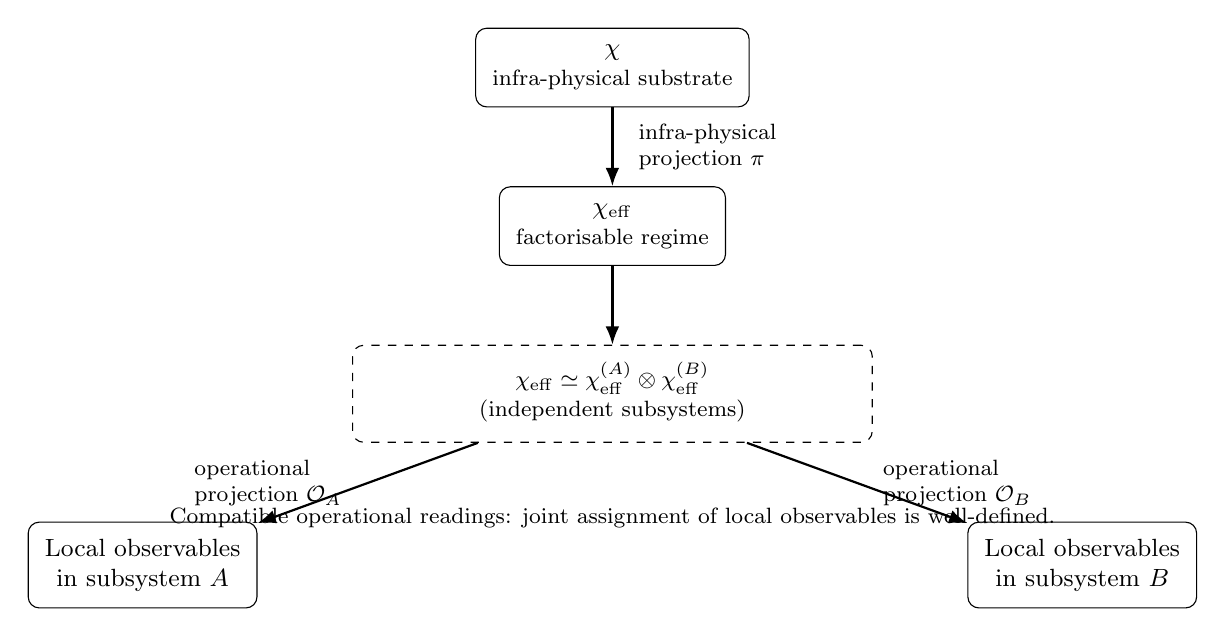
\begin{tikzpicture}[
      font=\small,
      node distance=10mm,
      box/.style={draw, rounded corners, align=center, inner sep=6pt},
      arrow/.style={-Latex, thick},
      note/.style={align=left, font=\footnotesize},
      dashedbox/.style={draw, dashed, rounded corners, inner sep=6pt}
    ]

    \node[box] (chi) {$\chi$\\\footnotesize infra-physical substrate};

    \node[box, below=of chi] (chieff) {$\chi_{\mathrm{eff}}$\\\footnotesize factorisable regime};

    \node[dashedbox, below=of chieff, minimum width=6.6cm] (decomp) {
      \begin{tabular}{c}
        \footnotesize $\chi_{\mathrm{eff}} \simeq \chi_{\mathrm{eff}}^{(A)} \otimes \chi_{\mathrm{eff}}^{(B)}$\\
        \footnotesize (independent subsystems)
      \end{tabular}
    };

    \node[box, below left=10mm and 12mm of decomp] (obsA) {Local observables\\in subsystem $A$};
    \node[box, below right=10mm and 12mm of decomp] (obsB) {Local observables\\in subsystem $B$};

    \draw[arrow] (chi) -- node[right=2mm, note] {infra-physical\\projection $\pi$} (chieff);
    \draw[arrow] (chieff) -- (decomp);

    \draw[arrow] (decomp) -- node[left=2mm, note] {operational\\projection $\mathcal{O}_A$} (obsA);
    \draw[arrow] (decomp) -- node[right=2mm, note] {operational\\projection $\mathcal{O}_B$} (obsB);

    \node[note, below=7mm of decomp, align=center] (compat)
    {\footnotesize Compatible operational readings: joint assignment of local observables is well-defined.};

    \end{tikzpicture}
    \caption{Classical (factorisable) regime. After the infra-physical projection $\pi$, the effective reality $\chi_{\mathrm{eff}}$ admits an approximate decomposition into independent subsystems. Operational projections $\mathcal{O}_A$ and $\mathcal{O}_B$ yield compatible local observables, recovering standard classical and relativistic descriptions in stable projectable domains.}
    \label{fig:classical-factorisable}
  \end{figure}

  In regimes where projected $\chi$ configurations exhibit sufficiently stable and
  smooth correlation patterns, variations of the effective scalar descriptor
  $\chi_{\mathrm{eff}}$ give rise to a set of operational observables.
  Because the projection from $\chi$ to $\chi_{\mathrm{eff}}$ is generically
  non-injective, these observables summarize relational structure without exhausting
  the underlying degrees of freedom.
  In particular, an increase in $\chi_{\mathrm{eff}}$ along a given physical process
  is associated with:
  \begin{itemize}
    \item the accumulation of operational proper time along that process,
    \item the progressive decorrelation between effective configurations, summarized
    as an emergent spatial separation,
    \item the large-scale expansion behavior observed when the ordering of projected
    $\chi$ configurations is considered at the cosmological level.
  \end{itemize}

  Within this effective description, temporal duration and spatial separation are not
  independent primitives.
  They represent complementary aspects of the same underlying ordering and relaxation
  structure, captured at different levels of coarse-graining.
  Heuristically, effective distance may be viewed as the persistent imprint of
  relational differentiation that has already occurred, while effective time
  corresponds to the ongoing local ordering of projected $\chi$ configurations.
  These expressions are intended as interpretative guides rather than literal
  definitions, emphasizing their common dynamical origin.

  This unified interpretation is not introduced \emph{ad hoc}.
  It follows directly from identifying temporal ordering, relational separation, and
  cosmological expansion as distinct effective summaries of the same irreversible
  $\chi$ dynamics, once a macroscopic spacetime description becomes appropriate.
  The physical content of the theory therefore resides entirely in the dynamics of the
  fundamental $\chi$ substrate, while spacetime notions serve only as emergent,
  context-dependent descriptive tools.

\subsection{Monotonicity and Arrow of Time}
\label{subsec:monotonicity-and-arrow-of-time}

A fundamental postulate of the theory is that $\chi$ evolves monotonically\cite{Prigogine1997,Penrose1989Weyl}:
\begin{equation}
  \frac{\partial \chi}{\partial t} \ge 0 .
\end{equation}

This monotonicity is not derived from statistical considerations but is taken as a primitive geometric property.
It provides a natural origin for the arrow of time and ensures global causal ordering without invoking special
boundary conditions.

Irreversibility arises because any decrease of $\chi$ would correspond to a contraction of both temporal and spatial
structure, which is dynamically forbidden within the theory.

\subsection{Local Relaxation Speed}
\label{subsec:local-relaxation-speed}

The local rate of change of $\chi$ is bounded by a universal constant:
\begin{equation}
  \left| \nabla_\mu \chi \right| \le c ,
\end{equation}
where $c$ coincides with the observed speed of light.

This bound does not represent the propagation speed of particles or signals, but the maximal rate at which
spacetime itself can locally unfold.
Superluminal recession velocities at cosmological scales arise naturally through cumulative effects and do not
violate local causality.

\subsection{Relation to Conventional Fields}
\label{subsec:relation-to-conventional-fields}

Although $\chi$ shares mathematical similarities with scalar fields used in cosmology (e.g., inflaton-like fields),
its role is fundamentally different.
It does not carry energy in the conventional sense, nor does it require quantization at the fundamental level.

Matter, radiation, and interactions emerge as localized excitations, constraints, or topological features of $\chi$,
rather than as independent entities coupled to it.

\subsection{Initial Conditions and Global Structure}
\label{subsec:initial-conditions-and-global-structure}

The theory assumes an initial condition characterized by a minimal value $\chi_0$, naturally associated with the Planck
scale.
Cosmic evolution corresponds to the progressive relaxation of $\chi$ from this initial state.

Importantly, the framework does not require a spacetime singularity in the traditional sense.
Instead, the apparent singular behavior arises from extrapolating classical notions of time and distance beyond the
domain where $\chi$ is well-defined.

In the next section, we derive a minimal dynamical equation governing the evolution of $\chi$ and explore its immediate
consequences.


  \input{04-chi-ontology/chi-ontology}
  \section{Dynamical Equation for the $\chi$ Field}
  \label{sec:dynamical-equation-for-the-chi-field}

  \input{04-chi-equation/01-parameter-independent-relaxation}
  \subsection{Hamiltonian Derivation of the Evolution Equation}
  \label{subsec:hamiltonian-derivation}

  \subsubsection*{Discrete Dynamics of $\chi$}
    Before introducing any metric structure, the dynamics of $\chi$ can be formulated purely in terms of its local
    relaxation on a discrete network.
    Let $\lambda$ be a monotonic ordering parameter, and define the local variation of $\chi$ at node $i$ as:
    \[
      \frac{d \chi_i}{d \lambda} = c \sqrt{1 - \frac{1}{c^2} \sum_{j \sim i} K_{ij} (\chi_i - \chi_j)^2}
      \label{eq:discrete-dynamics}
    \]
    Here, $K_{ij}$ is the connectivity strength between nodes $i$ and $j$ (introduced in
    Section~\ref{subsec:the-geometric-effective-action-and-lagrangians-of-cosmochrony-Lcc}), and the sum runs over
    neighboring nodes $j$.
    This equation is \textbf{metric-independent} and defines the fundamental dynamics of $\chi$ in terms of its local
    correlations.

  \subsubsection*{Continuum Limit}
    In the limit where the network becomes dense (i.e., the distance between nodes approaches zero), the discrete sum
    can be approximated by a continuous Laplacian:
    \[
      \sum_{j \sim i} K_{ij} (\chi_i - \chi_j)^2 \approx \int |\nabla \chi|^2 \, dV
    \]
    This yields the effective evolution equation in the continuum:
    \[
      \partial_t \chi = c \sqrt{1 - \frac{|\nabla \chi|^2}{c^2}}
    \]
    where $\nabla$ is now defined with respect to the emergent metric $g_{\mu\nu}$, derived from the network's
    connectivity (see Section~\ref{subsec:the-geometric-effective-action-and-lagrangians-of-cosmochrony-Lcc}).

  \subsubsection*{Hamiltonian Constraint}
    While the dynamics of $\chi$ can be viewed as a minimal relaxation principle, it can be more rigorously derived from
    a Hamiltonian constraint.
    We postulate that the dynamics of $\chi$ are governed by a Dirac-type kinematic constraint in phase space, analogous
    to the mass-shell condition for a massless relativistic particle:
    \[
      (\partial_t \chi)^2 + |\nabla \chi|^2 = c^2
      \label{eq:hamiltonian_constraint}
    \]
    where $c$ is the fundamental velocity scale.
    Combined with the arrow of time postulate ($\partial_t \chi \geq 0$), which reflects the irreversible relaxation of
    the Cosmochron, this leads uniquely to the first-order evolution equation:
    \[
      \partial_t \chi = c \sqrt{1 - \frac{|\nabla \chi|^2}{c^2}}
      \label{eq:chi_dynamics}
    \]
    This derivation grounds the ``minimal principle'' in the symplectic structure of the field's phase space, ensuring
    that $\chi$ acts as an intrinsic time coordinate.

  \subsection{Variational Formulation and Born-Infeld Action}
  \label{subsec:variational-formulation}

  To extend this kinematic constraint to a full dynamical theory including matter, we propose an effective Lagrangian
  density of the Born-Infeld type:
  \begin{equation}
    \mathcal{L} = -c^2 \sqrt{1 - \frac{|\nabla \chi|^2}{c^2}} + \partial_t \chi - \frac{4\pi G}{c^2} \rho \chi ,
  \end{equation}
  where $\rho$ represents the matter density. The presence of the term $\partial_t \chi$ linear in the first-order
  temporal derivative is crucial: it ensures that the momentum conjugate to $\chi$, defined as
  $\Pi_\chi = \frac{\partial \mathcal{L}}{\partial (\partial_t \chi)}$, is a non-vanishing constant ($\Pi_\chi = 1$).

  In the Hamiltonian formalism, this constant momentum acts as a primary constraint that effectively enforces the
  unit-velocity evolution of the field.
  This structure ensures that the field dynamics remain locked onto the Hamiltonian
  constraint~\eqref{eq:hamiltonian_constraint} while the square-root term acts as a non-linear regularizer for spatial
  gradients.
  The variation with respect to $\chi$ yields a non-linear Poisson equation:
  \begin{equation}
    \nabla \cdot \left( \frac{\nabla \chi}{\sqrt{1 - |\nabla \chi|^2/c^2}} \right) = \frac{4\pi G}{c^2} \rho .
    \label{eq:nonlinear_poisson}
  \end{equation}
  This formulation naturally recovers the Newtonian limit for weak gradients ($|\nabla \chi| \ll c$) while preventing
  gravitational singularities as the gradient magnitude is bounded by $c$.

  \subsection{Causality and Locality}
  \label{subsec:causality-and-locality}

  Equation~\eqref{eq:chi_dynamics} is explicitly local and causal.
  The evolution of $\chi$ at any spacetime point depends only on its immediate neighborhood through $\nabla \chi$.

  Importantly, no superluminal propagation occurs at the fundamental level.
  Apparent superluminal recession velocities in cosmology arise from integrating local $\chi$
  increments across extended regions, consistent with relativistic causality.

  \subsection{Homogeneous Cosmological Limit}
  \label{subsec:homogeneous-cosmological-limit}

  In a spatially homogeneous and isotropic configuration, $\nabla \chi = 0$
  , and the evolution equation simplifies to:
  \begin{equation}
    \partial_t \chi = c .
  \end{equation}

  This implies a linear growth\cite{Friedmann1922,Lemaitre1927}:
  \begin{equation}
    \chi(t) = \chi_0 + c t ,
  \end{equation}

  where $\chi_0$ denotes the initial value of $\chi$.

  This simple relation already reproduces a Hubble-like expansion law when distances are identified with accumulated
  $\chi$ increments, as discussed in Section~\ref{sec:cosmology}.

  As shown in Appendix~\ref{sec:mond_derivation}, the requirement $\partial_t \chi \geq 0$ in an expanding background
  ($H_0$) implies a minimal residual gradient $\nabla \chi_{\min} \propto \sqrt{H_0}$.
  This ``acceleration floor'' provides a first-principles derivation for MOND-like phenomenology, explaining galactic
  rotation curves without invoking dark matter particles.

  \subsection{Influence of Local Structure}
  \label{subsec:influence-of-local-structure}

  In regions where $\nabla \chi \neq 0$, the effective rate of $\chi$-relaxation is reduced.
  This slowing plays a central role in the emergence of gravitational phenomena.

  Localized excitations---identified with particles---act as topological or dynamical constraints on $\chi$,
  increasing $|\nabla \chi|$ and thereby locally reducing $\partial_t \chi$.

  This mechanism leads naturally to time dilation and spatial curvature without invoking an independent
  gravitational field.

  \input{04-chi-equation/07-unified-origin}
  \subsection{Limitations and Scope}
  \label{subsec:limitations-and-scope}

  Equation~\eqref{eq:chi_dynamics} is intentionally minimal.
  It does not attempt to describe quantum fluctuations of $\chi$, nor does it incorporate backreaction effects beyond
  first order.

  Its purpose is to provide a unified kinematic backbone from which gravitational, quantum, and cosmological
  phenomena can be derived consistently.

  In the following sections, we apply this dynamical framework to particles, gravity, and entanglement.


  \clearpage

\section{Particles as Localized Excitations of the
\texorpdfstring{$\chi$}{χ} Field}
\label{sec:particles-as-localized-excitations-of-the-chi-field}

% ----------------------------------------------------------------------------
% Section 4.1 --- Particles as Stable Wave Configurations
% From former §6.1
% ----------------------------------------------------------------------------
\subsection{Particles as Stable Wave Configurations}
\label{subsec:particles-as-stable-wave-configurations}

Particles are not fundamental point-like entities.
They arise at the level of effective descriptions as stable, localized
configurations within projected $\chi$
descriptions~\cite{Rajaraman1982}.
Such configurations correspond to persistent patterns that locally
constrain the admissible relaxation ordering.
In effective geometric regimes, they may be described using soliton-like
language.
Their stability reflects localized regions in which further relaxation is
strongly inhibited.
Apparent particle propagation corresponds to a continuous reorganization
of admissible projected descriptions, not to the motion of an object
through a fundamental spacetime.

\subsection{Topological Stability}
\label{subsec:topological-stability}

The stability of particle-like excitations does not rely on fundamental
conserved charges postulated \emph{a priori}.
Certain projected configurations exhibit non-trivial internal organization
that prevents them from being continuously deformed into homogeneous
effective descriptions without violating admissibility conditions.

This stability is topological in character: it reflects the existence of
inequivalent classes of admissible projected configurations that cannot be
smoothly connected through continuous reconfiguration while preserving
monotonic relaxation ordering.
The long-lived character of solitonic structures follows from this
topological incompatibility, not from a dynamical balance of forces.

Detailed geometric constructions of topological solitons, including
vortex, skyrmion, and knotted configurations, are provided in
Appendix~\ref{app:topological_solitons}.
The fully relational formulation is developed in
Appendix~\ref{app:relational_topological_stability}.

\subsection{Mass as Resistance to \texorpdfstring{$\chi$}{χ} Relaxation}
\label{subsec:mass_as_resistance}

Building on the ontological interpretation of mass as frozen structural
information (Section~\ref{subsec:mass-as-frozen-information}), we develop
the quantitative formulation.
Mass emerges at the effective level as a measure of how strongly a
localized projected configuration resists admissible relaxation ordering.

The effective structural energy associated with a projected solitonic
configuration $\chi_{\mathrm{eff},s}$ is
\begin{equation}
  E[\chi_{\mathrm{eff},s}] \;\equiv\;
  \int_{\Sigma}
  \left(
    \frac{1}{\sqrt{1
      - |\nabla \chi_{\mathrm{eff},s}|^2 / c^2}} - 1
  \right)
  \, d\Sigma ,
  \label{eq:chi_soliton_energy}
\end{equation}
where $\Sigma$ denotes a hypersurface of constant effective ordering
parameter and $|\nabla \chi_{\mathrm{eff},s}|$ quantifies effective
structural deformation.
The inertial mass is then defined operationally as
\begin{equation}
  m \;\equiv\; \frac{E[\chi_{\mathrm{eff},s}]}{c^2}.
  \label{eq:mass_definition}
\end{equation}
For example, the electron mass~$m_e$ reflects its topological stability as
a $4\pi$-periodic soliton
(Section~\ref{subsec:4pi_soliton}), while the proton mass arises from a
composite 3-soliton configuration.

The relation $E = mc^2$ is interpreted as a kinematic identity: mass
quantifies relaxation resistance, while energy expresses the same quantity
in relaxation units.
The question of how distinct particle masses arise from different classes
of projected configurations is addressed in
Appendix~\ref{app:topological_solitons}.

% ----------------------------------------------------------------------------
% Section 4.4 --- Metastability, Projection, and Particle Decay
% From former §6.4, condensed
% ----------------------------------------------------------------------------
\subsection{Metastability, Projection, and Particle Decay}
\label{subsec:metastability-and-decay}

A stable particle corresponds to a deep basin of admissible projected
configurations; an unstable particle occupies a shallow or fragile basin.
Particle decay is interpreted as the structural reorganization of a
metastable configuration: when the concentration of constraints exceeds
what can be sustained by a single projected entity, admissibility is
recovered through factorization into less constrained localized
configurations, possibly accompanied by weakly structured excitations.

Entanglement and decay represent two regimes of the same projection
structure.
Entanglement corresponds to non-factorizability without fragmentation,
while decay corresponds to non-factorizability that forces fragmentation.
The distinction lies in the stability properties of the projected
description under admissible fluctuations.

The finite lifetime of unstable particles reflects the probability of
crossing a structural reorganization threshold under admissible
variations, yielding the observed exponential decay law as a statistical
signature of metastability.

\begin{figure}[t]
  \centering
  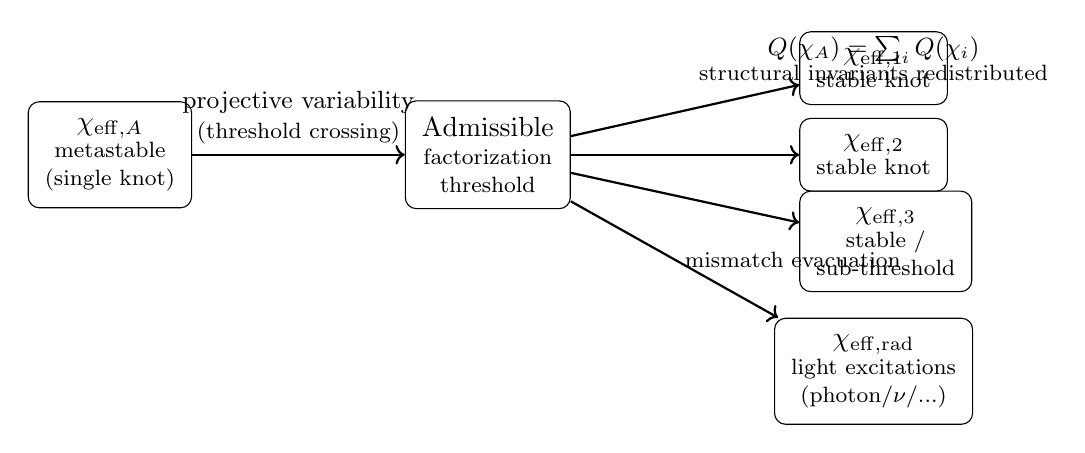
\begin{tikzpicture}[
    box/.style={draw, rounded corners, align=center, inner sep=6pt},
    arr/.style={->, thick},
    lab/.style={font=\small, align=center}
  ]
    \node[box] (A)
      {$\chi_{\mathrm{eff},A}$\\[-2pt]\footnotesize metastable\\
       [-2pt]\footnotesize (single knot)};
    \node[box, right=2.7cm of A] (T)
      {Admissible\\[-2pt]\footnotesize factorization\\
       [-2pt]\footnotesize threshold};
    \node[box, right=2.9cm of T, yshift=1.1cm] (B1)
      {$\chi_{\mathrm{eff},1}$\\[-2pt]\footnotesize stable knot};
    \node[box, right=2.9cm of T] (B2)
      {$\chi_{\mathrm{eff},2}$\\[-2pt]\footnotesize stable knot};
    \node[box, right=2.9cm of T, yshift=-1.1cm] (B3)
      {$\chi_{\mathrm{eff},3}$\\[-2pt]\footnotesize stable /\\
       [-2pt]\footnotesize sub-threshold};
    \node[box, below=1.6cm of B2] (R)
      {$\chi_{\mathrm{eff,rad}}$\\[-2pt]\footnotesize light
       excitations\\[-2pt]\footnotesize (photon/$\nu$/...)};
    \draw[arr] (A) -- node[lab, above]
      {projective variability\\
       \footnotesize (threshold crossing)} (T);
    \draw[arr] (T) -- (B1);
    \draw[arr] (T) -- (B2);
    \draw[arr] (T) -- (B3);
    \draw[arr] (T) -- node[lab, right]
      {\footnotesize mismatch evacuation} (R);
    \node[lab, above=0.35cm of B2] (Q)
      {$Q(\chi_A)=\sum_i Q(\chi_i)$\\[-2pt]
       \footnotesize structural invariants redistributed};
  \end{tikzpicture}
  \caption{Structural interpretation of particle decay.
    A metastable localized projected configuration transitions, via an
    admissible factorization threshold, into several more stable
    configurations plus weak excitations that evacuate the residual
    structural mismatch.}
  \label{fig:decay-fragmentation}
\end{figure}

A more technical characterization of metastability, admissible
factorization channels, and decay widths is provided in
Appendix~\ref{subsec:metastability-decay-channels-and-exponential-lifetimes}.

% ----------------------------------------------------------------------------
% Section 4.5 --- Energy--Frequency Relation
% From former §6.5
% ----------------------------------------------------------------------------
\subsection{Energy--Frequency Relation}
\label{subsec:energy-frequency-solitons}

The energy associated with a particle-like excitation is linked to a
characteristic internal spectral scale of the corresponding projected
configuration.
Configurations associated with higher characteristic frequencies
correspond to more tightly constrained structures and encode greater
effective resistance to relaxation.
This yields
\begin{equation}
  E \propto \nu ,
\end{equation}
where $\nu$ characterizes the spectral scale of internal organization.
Planck's constant appears as an effective proportionality factor whose
universality reflects the robustness of spectral scales in the current
relaxation epoch.
A more explicit realization in the context of radiation is presented in
Section~\ref{subsec:energy-frequency-radiation}.

% ----------------------------------------------------------------------------
% Section 4.6 --- Fermions, Bosons, and Spin
% Merges former §6.6 and §6.7
% ----------------------------------------------------------------------------
\subsection{Fermions, Bosons, and Spin}
\label{subsec:fermions-and-bosons}

Particle statistics emerge from the topological structure of admissible
projected configurations.
Configurations requiring a $4\pi$ rotation to return to an equivalent
projected description give rise to fermion-like behavior, while
$2\pi$-periodic configurations correspond to bosons.
This distinction reflects a topological obstruction rather than a symmetry
principle imposed at the fundamental level.

\subsubsection*{Spin as a Topological Property}
\label{subsec:spin_topology}

Spin is not an intrinsic kinematic degree of freedom but a purely
topological property of admissible projected configurations.
Fermionic configurations require a $4\pi$ transformation in configuration
space to return to an equivalent effective description, implying that the
relevant configuration space admits a double covering with fundamental
group
\begin{equation}
  \pi_1(\mathcal{C}_{\mathrm{eff}}) = \mathbb{Z}_2 .
\end{equation}

When an effective quantum description is applicable, a $2\pi$
transformation induces a sign change of the associated wavefunction,
\begin{equation}
  \psi \;\longrightarrow\; -\psi ,
\end{equation}
while a $4\pi$ transformation restores the original state.
This $4\pi$-periodicity directly implies fermionic antisymmetry and the
Pauli exclusion principle, as detailed in
Section~\ref{app:relational_spin_statistics}.

Exchanging two identical fermionic excitations corresponds topologically
to a $2\pi$ loop in the combined configuration space and induces a sign
change, dynamically excluding symmetric
configurations~\cite{Pauli1925}.
The spin--statistics connection thus admits a unified topological origin
within the effective descriptive framework.

\input{2-dynamics_and_particles/04-particles-as-localized-excitations-of-the-chi-field/sec-charge}
% ----------------------------------------------------------------------------
% Section 4.8 --- Antiparticles, Creation/Destruction, and CPT
% Merges former §6.9, §6.10, §6.11, heavily condensed
% ----------------------------------------------------------------------------
\subsection{Antiparticles, Creation/Destruction, and CPT}
\label{subsec:antiparticles}

\subsubsection*{Antiparticles as Relationally Conjugate Configurations}

A particle and its antiparticle correspond to projected configurations
belonging to distinct but conjugate topological classes within the space
of admissible projected descriptions, related by an internal reversal of
relational organization.
Annihilation occurs when a particle-like configuration and its conjugate
combine into a composite description that no longer supports localized
structural constraints, redistributing relational structure into
delocalized radiation-like excitations.
This constitutes a process of \emph{structural unknotting}: mass itself
measures the degree of topological obstruction to relaxation.

\paragraph{Why Antimatter Does Not Require Time Reversal.}
\label{subsec:why-antimatter-no-time-reversal}
The monotonic ordering of~$\chi$ defines an absolute arrow of admissible
projection that cannot be inverted.
Antiparticles correspond to topologically conjugate classes, not to
reversed temporal trajectories.
The apparent association between antimatter and time reversal in standard
formalisms is a feature of the effective representation.

\paragraph{Matter--Antimatter Asymmetry without Fundamental CP Violation.}
\label{subsec:matter-antimatter-asymmetry-without-cp}
If the projection from~$\chi$ to effective spacetime is chiral, conjugate
classes need not be realized with equal stability or projectability.
Matter--antimatter asymmetry emerges as a selection effect imposed by
differential projectability, without requiring dynamical CP-breaking
interactions.

\subsubsection*{Particle Creation and Destruction}
\label{subsec:particle-creation-and-destruction}

Particle creation corresponds to a projected configuration acquiring
sufficient structural organization to support a stable topological class.
Particle destruction occurs when a configuration loses its topological
admissibility and admits continuous deformation toward a delocalized
effective description.

\subsubsection*{CPT as a Global Projective Property}
\label{subsec:cpt-as-global-projective-property}

C, P, and T are individually effective and representation-dependent.
Their combined action corresponds to a full relational conjugation of
projected descriptions, mapping any admissible effective configuration to
another admissible configuration representing the same underlying
$\chi$ structure.
CPT invariance is therefore not a microscopic symmetry but a global
projective consistency condition ensuring that the space of admissible
descriptions is closed under full relational conjugation.
Violations of CPT would signal a breakdown of projectability itself.

\subsubsection*{CPT as an Admissibility Consistency Condition}
\label{subsec:antiparticles-cpt}

Certain projected configurations carry orientation-sensitive structural
invariants (chirality, phase winding, relational orientation).
Under admissible factorization, these signed invariants must be
redistributed, possibly requiring paired localized excitations carrying
opposite orientations---interpreted as particle--antiparticle pairs.
CPT symmetry reflects the invariance of admissibility under a combined
reversal of signed structural invariants, effective spatial orientation,
and the effective ordering parameter.
A technical formulation is provided in
Appendix~\ref{subsec:structural-interpretation-of-cpt-symmetry}.

\paragraph{Why CPT Survives Quantum Gravity.}
\label{subsec:why-cpt-survives-quantum-gravity}
CPT survives because it expresses the minimal requirement for a coherent
physical projection.
Quantum gravity may challenge locality, geometry, and the notion of time,
but cannot violate CPT without undermining the possibility of a
consistent emergent universe.

% ----------------------------------------------------------------------------
% Section 4.9 --- Neutrinos as Partially Projectable Modes
% From former §6.12, drastically condensed
% ----------------------------------------------------------------------------
\subsection{Neutrinos as Partially Projectable Modes}
\label{subsec:neutrinos-partially-projectable-modes}

Neutrinos correspond to \emph{partially projectable modes} of~$\chi$:
configurations whose relational structure admits a stable projection in
some degrees of freedom while remaining weakly or non-projectable in
others.
This partial projectability explains their extremely small effective
masses, weak interaction strength, and sensitivity to global rather than
local structural properties of the projection.

\paragraph{Dirac vs.\ Majorana Character.}
A Dirac neutrino admits distinct conjugate projected realizations; a
Majorana neutrino corresponds to a configuration whose partial
projectability collapses the distinction between conjugate classes.
The Dirac or Majorana character is not a fundamental choice but a
manifestation of how fully the projection resolves relational
conjugation.
Lepton number conservation emerges only in regimes where conjugate
configurations are distinguishable; when partial projectability erases
this distinction, effective lepton number violation becomes admissible.

\paragraph{Neutrino Oscillations without Fundamental Mass Eigenstates.}
\label{subsec:neutrino-oscillations-without-mass-eigenstates}
Different flavors correspond to closely related partially projectable
configurations whose internal relational structures overlap but are not
identical.
As projected descriptions evolve along the monotonic ordering of~$\chi$,
the relative projectability of these configurations varies, leading to
coherent transitions between flavor labels without invoking mass
eigenstates as fundamental objects.

\paragraph{Stability of the Projection Boundary.}
\label{subsec:neutrinos-and-projection-boundary-stability}
Neutrinos occupy an intermediate regime between fully localized particles
and delocalized radiation.
They act as carriers of marginal structural information, redistributing
relational organization without inducing strong backreaction, thereby
preventing abrupt transitions between projectable and non-projectable
regimes.
In strong-gravity or near-deprojection regimes, neutrinos remain among
the last modes to retain partial projectability.

\paragraph{Why Neutrinos Are the Lightest Fermions.}
\label{subsec:why-neutrinos-are-lightest-fermions}
Neutrino configurations reside closest to the boundary of
projectability.
Their absence of electromagnetic coupling and partial self-conjugacy
prevent the formation of tightly bound projected structures.
The smallness of neutrino masses is a structural necessity imposed by
their role as marginally projectable modes.

\paragraph{Neutrinos as Probes of Pre-Geometric Structure.}
\label{subsec:neutrinos-as-probes-of-pregeometric-structure}
Because neutrinos operate near the projection boundary, they provide a
unique observational window into the pre-geometric structure of~$\chi$.
Their weak localization allows them to sample relational structures
inaccessible to fully projectable modes, and deviations in their
phenomenology may encode signatures of pre-geometric ordering.

\paragraph{Failure of Absolute Localization.}
\label{subsec:neutrinos-failure-of-absolute-localization}
Neutrinos cannot be fully confined within a bounded spacetime region
without loss of admissibility, explaining their absence of sharply
defined position operators and extremely small interaction
cross-sections.

\paragraph{Limits of Effective Quantum Field Theory.}
\label{subsec:neutrinos-limits-of-qft}
Neutrinos systematically probe the limits of local QFT assumptions.
Their weak localization, extended coherence, and oscillatory behavior
signal a breakdown of the strict particle ontology.
Standard QFT constructs (mass eigenstates, flavor mixing matrices) are
understood as effective bookkeeping devices for marginally projectable
configurations.

\paragraph{Experimental Signatures.}
\label{subsec:experimental-signatures-projective-neutrinos}
Potential signatures include small departures from standard oscillation
patterns at ultra-long baselines, coherence and decoherence effects
sensitive to global spacetime properties, constraints from neutrinoless
double beta decay on the projective resolution of conjugate
configurations, and cosmological neutrino backgrounds encoding
information about the approach to the projection boundary.

\paragraph{Synthesis.}
\label{subsec:synthesis-neutrinos-structural-frontier}
Neutrinos mark the transition between physics described by local quantum
fields on spacetime and the pre-geometric relational dynamics of~$\chi$.
They constitute the structural frontier of emergent spacetime, where
effective geometry, quantum description, and pre-geometric ontology
converge.

\input{2-dynamics_and_particles/04-particles-as-localized-excitations-of-the-chi-field/sec-lamb-shift}
% ----------------------------------------------------------------------------
% Section 4.11 --- Summary
% From former §6.14, condensed
% ----------------------------------------------------------------------------
\subsection{Summary}
\label{subsec:summary-particles}

Particles arise as stable, localized projected configurations that resist
admissible relaxation ordering.
Mass is identified with the degree of effective resistance to $\chi$
relaxation, naturally yielding $E = mc^2$ as a kinematic identity.
Spin and statistical behavior originate from topological obstructions:
fermionic configurations exhibit $4\pi$ periodicity, providing a unified
origin for spin-$\tfrac{1}{2}$ behavior, fermionic antisymmetry, and the
Pauli exclusion
principle~\cite{Pauli1925,Dirac1928}.
Electric charge is interpreted as a chiral--torsional invariant of the
relaxation flux.
Residual spectral splittings---such as the Lamb shift and hyperfine
structure---arise as finite corrections induced by non-linear saturation
and projectability constraints.


  \clearpage

\section{Gravity as a Collective Effect of Particle Excitations}
\label{sec:gravity-as-a-collective-effect-of-particle-excitations}

\input{3-gravitation-and-cosmology/06-gravity-as-a-collective-effect-of-particle-excitations/001-local-slowdown}
\subsection{Collective Gravitational Coupling and Operational Geometry}
  \label{subsec:collective-gravitational-coupling-and-operational-geometry}

  The collective reduction of admissible relaxation ordering modulates how
  efficiently structural variations can be correlated between different
  effective locations.
  In regions where projected descriptions are nearly homogeneous, the
  effective coupling approaches a uniform value; localized configurations
  weaken it by introducing structural constraints.

  From an operational perspective, this modulation can be interpreted as a
  \emph{self-consistency overhead}: maintaining mutual compatibility of
  projected descriptions across separated regions requires an increasing
  consistency cost as local constraints accumulate.
  Inertial and gravitational responses arise precisely as manifestations of
  this overhead in collective updates of the effective state.

  Spatial separation is defined operationally: two effective regions are
  close if structural variations can be efficiently correlated between
  them.
  In the continuum and weak-constraint regime, this operational notion
  admits a compact description in terms of an effective spatial metric
  summarizing the collective response to relative variations.
  Spacetime curvature emerges as a descriptive manifestation of how
  localized configurations modulate collective ordering, correlation
  efficiency, and the associated self-consistency overhead.

  A more explicit relational construction of the coupling mechanism is
  presented in Appendix~\ref{subsec:collective-coupling}.

\input{3-gravitation-and-cosmology/06-gravity-as-a-collective-effect-of-particle-excitations/003-emergent-curvature}
\input{3-gravitation-and-cosmology/06-gravity-as-a-collective-effect-of-particle-excitations/004-schwarzschild}
% ----------------------------------------------------------------------------
% Section 6.5 --- Equivalence Principle
% From former §7.5, condensed
% ----------------------------------------------------------------------------
\subsection{Equivalence Principle}
\label{subsec:equivalence-principle}

All admissible localized projected configurations constrain relaxation
ordering in the same universal manner.
Their internal composition plays no role in how they affect or respond to
the admissible ordering environment.
Inertial resistance and gravitational response are two effective
manifestations of the same underlying constraint, and the equivalence
principle arises as an emergent symmetry of admissible projected
descriptions.

\input{3-gravitation-and-cosmology/06-gravity-as-a-collective-effect-of-particle-excitations/006-gravitational-waves}
\input{3-gravitation-and-cosmology/06-gravity-as-a-collective-effect-of-particle-excitations/007-strong-gravity-bh}
\input{3-gravitation-and-cosmology/06-gravity-as-a-collective-effect-of-particle-excitations/008-bh-evaporation}
\input{3-gravitation-and-cosmology/06-gravity-as-a-collective-effect-of-particle-excitations/009-unified-grav-em}
\input{3-gravitation-and-cosmology/06-gravity-as-a-collective-effect-of-particle-excitations/010-lensing}
% ----------------------------------------------------------------------------
% Section 6.11 --- Summary
% From former §7.11, condensed
% ----------------------------------------------------------------------------
\subsection{Summary}
\label{subsec:summary-gravity}

Gravity emerges as a macroscopic consequence of localized projected
configurations collectively constraining admissible relaxation ordering.
Classical gravitational phenomena---time dilation, curvature,
gravitational waves, and black holes---are recovered as distinct
descriptive regimes of this collective constraint.
In extreme regimes, the spectral structure of horizon-associated phenomena
encodes direct information about the relaxation dynamics and projection
topology of the underlying substrate.


  \clearpage

\section{Quantum Phenomena and Entanglement}
  \label{sec:quantum-phenomena-and-entanglement}

  \paragraph{Scope and strategy.}
    This section explains how quantum phenomenology arises as an effective statistical
    description of the projection process in Cosmochrony.
    Building on the \emph{non-injectivity of the projection $\Pi$ established in
Section~\ref{sec:relational_projection}}, we show how entanglement, nonlocal
    correlations, and measurement statistics emerge without introducing additional
    ontological degrees of freedom.

    Distinct underlying $\chi$ configurations may correspond to identical effective
    observables, and a single relational configuration may admit multiple effective
    images depending on the operational context.
    We adopt an \textbf{ontological monism} viewpoint: there is a single ontological
    substrate $\chi$, while apparent multiplicity and spatial separation are properties
    of the projected description.

    Within this setting, so-called ``nonlocality'' does not involve signal transmission.
    Correlated outcomes do not originate from independent ontological subsystems, but
    from a shared underlying relational structure accessed through non-injective
    projection.

    \subsection{Non-Injective Projection as the Origin of Quantum Correlations}
  \label{subsec:non-injective-projection}

  The emergence of quantum correlations and entanglement in the Cosmochrony
  framework is rooted in a single structural property of the projection from
  the fundamental $\chi$ substrate to effective physical descriptions:
  this projection is \emph{non-injective}.

  A single admissible configuration of $\chi$ may correspond to multiple
  distinct effective degrees of freedom.
  What appear, at the effective level, as separate particles or subsystems
  are therefore multiple projective manifestations of a single underlying
  ontological configuration.

  This non-injectivity implies that such degrees of freedom cannot be assigned
  independent states.
  Any admissible effective description must be globally consistent with the
  underlying $\chi$ configuration, leading to persistent correlations that
  do not rely on signal exchange, causal influence, or spacetime proximity.

    \input{08-quantum-correlations-and-entanglement/02-nonlocality-and-holistic-nature}
    \subsection{Nonlocal Correlations Without Superluminality}
  \label{subsec:nonlocal-correlations-without-superluminality}

  Within the Cosmochrony framework, nonlocal quantum correlations do not arise from
  superluminal propagation of information.
  All admissible projected descriptions respect local causal constraints, and no
  measurement outcome influences another through dynamical signal exchange.

  This absence of superluminal influence follows directly from the non-injective
  character of the projection from the underlying $\chi$ substrate.
  Because spacelike separated outcomes correspond to distinct local reprojections
  of a single underlying configuration, no information transfer is required to account for their correlation.

  Correlated outcomes instead arise because spacelike separated measurements correspond
  to different local reprojections of a single non-factorizable admissible projected description.
  Such descriptions cannot be decomposed into independent subsystems without loss of global consistency.
  This failure of factorization is not accidental, but reflects the absence of an
  injective mapping between effective subsystems and underlying $\chi$ configurations.
  As a result, the factorization assumptions underlying Bell-type inequalities are
  violated, while dynamical locality and relativistic causality remain intact.
  This point is grounded in the relational formulation, where factorization is not
  fundamental but only an approximate emergent feature of certain projectable regimes
  (see Appendix~E, especially Appendix~\ref{subsec:non-factorization-and-entanglement}.

  In this perspective, quantum correlations reflect global descriptive consistency
  rather than hidden variables or pre-existing local properties.
  Measurement outcomes do not reveal predetermined values, but correspond to compatible
  local realizations selected from a shared non-factorizable descriptive structure.
  Equivalently, admissible projected descriptions determine a constrained \emph{space}
  of mutually compatible local realizations, rather than a set of pre-assigned outcomes.

  Cosmochrony therefore accounts for experimentally observed violations of Bell
  inequalities without invoking nonlocal forces, retrocausality, or hidden signal
  channels.
  Nonlocality appears as a structural feature of admissible projected descriptions,
  fully compatible with relativistic causal constraints.
  A compact way to state this is that the correlations are \emph{ontological}, fixed by the non-injective global
  relational structure, rather than \emph{dynamical}, mediated by any superluminal interaction.

    \subsection{Relation to Bell Inequalities}
  \label{subsec:relation-to-bell-inequalities}

  Bell's theorem~\cite{Bell1964} establishes that no physical theory reproducing the full
  set of quantum mechanical predictions can simultaneously satisfy locality,
  realism understood as outcome determinism conditioned on hidden variables, and statistical independence.
  The empirical violations of Bell inequalities therefore rule out any ontological
  completion of quantum mechanics based on factorizable hidden-variable models.

  The Cosmochrony framework fully accepts Bell's theorem as a fundamental constraint.
  It does not seek to evade or weaken Bell inequalities, nor to restore locality or realism in their classical sense.
  Instead, it identifies the precise ontological assumption that fails within
  Bell-type derivations when applied to admissible projected descriptions.

  \paragraph{Failure of ontological factorisability.}
    Standard Bell-type arguments assume that joint outcome probabilities admit a factorization of the form
    \begin{equation}
      P(a,b|x,y,\lambda) = P(a|x,\lambda)\,P(b|y,\lambda),
    \end{equation}
    where $\lambda$ denotes a complete specification of the underlying ontic state.
    In Cosmochrony, such a decomposition is not available, not because of nonlocal
    dynamical influences, but because admissible effective descriptions arise from
    \emph{non-injective projections} of the underlying $\chi$ substrate.

    Distinct fundamental configurations of $\chi$ may correspond to the same effective
    projected description, while remaining globally constrained.
    As a consequence, entangled systems correspond to equivalence classes of
    non-separable configurations that do not admit independent ontic pre-images for their subsystems.
    There exists no hidden variable $\lambda$ with respect to which conditional
    factorization could be restored, even in principle.

  \paragraph{No hidden variables and no superluminal influence.}
    The non-injectivity of the projection does not introduce hidden variables, local or nonlocal.
    The underlying degrees of freedom are neither accessible nor conditionable,
    and they cannot be used to screen correlations or define outcome-determining parameters.
    Accordingly, the violation of Bell inequalities in Cosmochrony does not rely on
    superluminal signalling, retrocausality, or a breakdown of relativistic causal structure.

    Correlations are not mediated, transmitted, or dynamically generated between spatially separated subsystems.
    They reflect global admissibility constraints on projected descriptions, inherited
    from the holistic structure of the underlying configuration space.

  \paragraph{Ontological rather than dynamical nonlocality.}
    In this sense, quantum nonlocality in Cosmochrony is ontological rather than dynamical.
    The failure of factorization arises from the structure of the projection map itself,
    not from any nonlocal interaction or exchange of information.
    Bell-type violations are therefore understood as a manifestation of the
    non-separable nature of admissible descriptions, rather than as evidence for superluminal influences.

    This interpretation preserves the full empirical content of quantum mechanics,
    respects relativistic causality at the operational level, and provides a structural
    explanation for the inevitability of entanglement correlations within a non-injective relational framework.

    \input{08-quantum-correlations-and-entanglement/05-measurement-and-decoherence}
    \input{08-quantum-correlations-and-entanglement/06-temporal-ordering-and-relativistic-consistency}
    \input{08-quantum-correlations-and-entanglement/07-limits-of-entanglement}
    \input{08-quantum-correlations-and-entanglement/08-standard-model-integration}
    \input{08-quantum-correlations-and-entanglement/09-summary}
    \subsection{Structural Stability of Projected Descriptions}
  \label{subsec:noninjective-projection-entanglement}

  Quantum entanglement, measurement, and decay correspond to distinct stability regimes
  of projected descriptions in Cosmochrony.
  Building on the non-injectivity of the projection $\Pi$ established in
  Section~\ref{sec:relational_projection}, we analyze how non-factorizable projected
  descriptions may remain stable, become unstable, or fragment into localized
  factorizable descriptions under admissible interactions and fluctuations.

  A single relational configuration of \(\chi\) may admit multiple effective
  descriptions that cannot be decomposed into independent subsystems without violating
  admissibility constraints.

  Quantum entanglement corresponds to the regime in which such a non-factorizable
  projected description remains structurally stable.
  Although effective observables may be associated with spatially separated regions, the
  projected configuration retains its unity and cannot be expressed as a product of
  independent components.
  Nonlocal correlations therefore reflect the relational character of the underlying
  \(\chi\)-configuration rather than any superluminal influence.

  Measurement and decoherence correspond to a selective stabilization within the space of
  admissible projected descriptions.
  Interaction with an environment amplifies certain relational features while rendering
  alternative projected descriptions inadmissible.
  The apparent collapse of the wavefunction thus reflects a loss of admissibility of
  non-selected descriptions, rather than a fundamental discontinuity at the level of the
  \(\chi\)-substrate.

  Particle decay represents a distinct but closely related regime.
  Here, the non-factorizable projected description becomes unstable under admissible
  fluctuations.
  No single projected configuration remains admissible, and stability is recovered only
  through factorization into several localized projected configurations.
  In this sense, decay may be understood as a structural transition from non-factorizable
  to factorizable projected descriptions.

  Entanglement, measurement, and decay therefore arise from a common structural origin:
  the stability properties of non-factorizable projected descriptions under admissible
  interactions and fluctuations.
  They differ not in the nature of the underlying $\chi$ substrate, but in the dynamical
  response of projected descriptions to perturbations within the admissible spectrum.

  \begin{figure}[t]
    \centering
    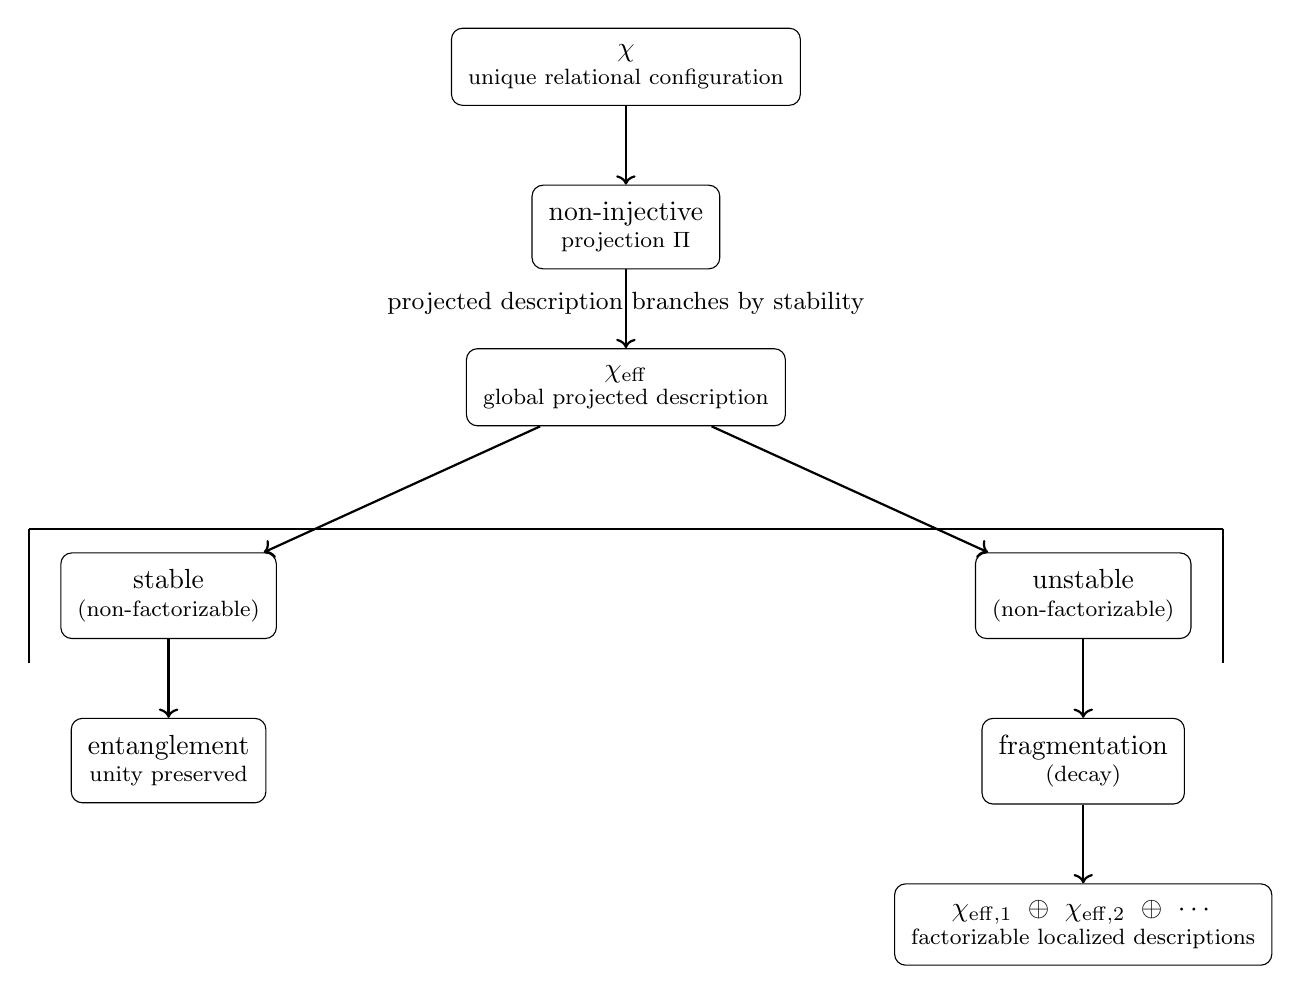
\begin{tikzpicture}[
      node distance=10mm and 18mm,
      box/.style={draw, rounded corners, align=center, inner sep=6pt},
      arr/.style={->, thick},
      lab/.style={font=\small, align=center},
      faint/.style={font=\small}
    ]

% Top chain
      \node[box] (chi) {$\chi$\\[-2pt]\footnotesize unique relational configuration};
      \node[box, below=of chi] (proj) {non-injective\\[-2pt]\footnotesize projection $\Pi$};
      \node[box, below=of proj] (chieff) {$\chi_{\mathrm{eff}}$\\[-2pt]\footnotesize global projected description};

% Split
      \node[box, below left=16mm and 24mm of chieff] (stable) {stable\\[-2pt]\footnotesize (non-factorizable)};
      \node[box, below right=16mm and 24mm of chieff] (unstable) {unstable\\[-2pt]\footnotesize (non-factorizable)};

% Outcomes
      \node[box, below=of stable] (ent) {entanglement\\[-2pt]\footnotesize unity preserved};
      \node[box, below=of unstable] (frag) {fragmentation\\[-2pt]\footnotesize (decay)};

      \node[box, below=of frag] (sum){$\chi_{\mathrm{eff},1}\ \oplus\ \chi_{\mathrm{eff},2}\ \oplus\ \cdots$
        \\[-2pt]\footnotesize factorizable localized descriptions};

% Arrows
      \draw[arr] (chi) -- (proj);
      \draw[arr] (proj) -- (chieff);

      \draw[arr] (chieff) -- (stable);
      \draw[arr] (chieff) -- (unstable);

      \draw[arr] (stable) -- (ent);
      \draw[arr] (unstable) -- (frag);
      \draw[arr] (frag) -- (sum);

% Bracket / grouping
      \draw[thick] ($(stable.north west)+(-4mm,3mm)$) -- ($(unstable.north east)+(4mm,3mm)$);
      \draw[thick] ($(stable.north west)+(-4mm,3mm)$) -- ($(stable.south west)+(-4mm,-3mm)$);
      \draw[thick] ($(unstable.north east)+(4mm,3mm)$) -- ($(unstable.south east)+(4mm,-3mm)$);

% Optional label above bracket
      \node[lab, above=3mm of chieff] {projected description branches by stability};
    \end{tikzpicture}
    \caption{Conceptual branching induced by non-injective projection in Cosmochrony.
    A single relational configuration of \(\chi\) may admit a global non-factorizable
    projected description. If this description is stable, it manifests as entanglement.
    If it is unstable, admissibility is recovered through fragmentation into multiple
    localized factorizable descriptions (particle decay).}
    \label{fig:noninjective-branching-entanglement-decay}
  \end{figure}

  A technical analysis of non-injective projection, admissibility conditions, and
  structural factorization is provided in
  Appendix~\ref{subsec:non-injective-projection-and-structural-factorization}.

    \subsection{Entanglement as a Critical Regime of Projective Compression}
  \label{subsec:entanglement-as-a-critical-regime-of-projective-compression}

\subsection{Entanglement as a Critical Regime of Projective Compression}
  \label{subsec:entanglement-critical-compression}

  Within the Cosmochrony framework, quantum entanglement is not introduced as a primitive
  feature of physical systems, nor as a purely formal property of Hilbert space states.
  Instead, it arises as a structural consequence of the non-injective projection
  $\Pi:\chi \rightarrow \chi_{\mathrm{eff}}$ that maps the relational substrate to effective descriptions.

  \paragraph{Projection as an information-compressive process.}
    The projection $\Pi$ reduces a high-dimensional relational configuration of $\chi$ to a
    lower-dimensional effective description by discarding unresolved internal degrees of freedom.
    As a result, a single effective configuration $\chi_{\mathrm{eff}}$ generally corresponds
    to an equivalence class of admissible underlying configurations, forming a projection
    fiber $\Pi^{-1}(\chi_{\mathrm{eff}})$.
    This fiber may be understood as an information-theoretic channel whose effective bandwidth
    is determined by the number and structure of unresolved modes of $\chi$.
    The non-injectivity of $\Pi$ thus corresponds to an intrinsic compression of relational
    information, rather than to epistemic ignorance or hidden variables.

  \paragraph{Compression and effective separability.}
    The degree of compression induced by $\Pi$ controls the structure of admissible projected descriptions.
    In the limit of negligible compression, the effective description retains too much
    microscopic relational detail to admit a stable decomposition into subsystems, and no
    robust notion of separability arises.
    Conversely, in the limit of extreme compression, most relational information is erased,
    and projected descriptions become effectively factorized, recovering classical statistical behavior.

    Crucially, non-factorizable correlations do not increase monotonically with the strength of compression.
    Instead, they emerge only within an intermediate regime in which the effective description
    is sufficiently coarse-grained to permit subsystem identification, yet retains enough
    global relational structure to prevent full factorization.

  \paragraph{Entanglement as a critical regime.}
    Quantum entanglement corresponds precisely to this intermediate, critical regime of projective compression.
    In this regime, distinct effective subsystems are well defined, but remain globally
    constrained by compatibility conditions inherited from the underlying relational configuration.
    As a result, joint outcome statistics fail to admit an ontologically factorizable
    representation, even though no dynamical interaction or information exchange occurs
    between spatially separated subsystems.

    This interpretation naturally explains why entanglement correlations are both robust and bounded.
    If compression is increased beyond the critical regime—through environmental coupling,
    decoherence, or coarse-graining—the effective description becomes over-compressed and
    correlations are suppressed, leading to classical behavior.
    If compression is reduced below the critical regime, effective subsystem separation
    breaks down and no stable notion of entanglement applies.

  \paragraph{Structural role of entanglement.}
    From this perspective, entanglement is neither a consequence of maximal information
    preservation nor of maximal information loss.
    Rather, it is a structural feature that emerges at the boundary between the two, as a
    manifestation of residual global constraints surviving projection.
    This view unifies the appearance of entanglement, its sensitivity to environmental
    effects, and its disappearance in the classical limit within a single relational and
    information-theoretic mechanism.

    Bell inequality violations, discussed in Section~\ref{subsec:relation-to-bell-inequalities}, follow necessarily from
    the failure of ontological factorization in this critical regime, and do not require the introduction of
    superluminal influences or hidden variables.


  \input{09-quantum-formalism/quantum-formalism}
  % ============================================================================
% Chapter 7 --- Cosmological Implications
% From former section 12 of Cosmochrony v1.13beta1, streamlined
% ============================================================================
\clearpage

\section{Cosmological Implications}
\label{sec:cosmology}

% ----------------------------------------------------------------------------
% Section 7.1 --- The Big Bang as a Maximal Constraint Regime
% From former §12.1, condensed
% ----------------------------------------------------------------------------
\subsection{The Big Bang as a Maximal Constraint Regime of the
\texorpdfstring{$\chi$}{χ} Substrate}
\label{subsec:big-bang-maximal-constraint}

The Big Bang is interpreted as the boundary of applicability of effective
spacetime descriptions.
In this regime, the density of structural and topological constraints
within~$\chi$ exceeds the threshold required for stable geometric
projection: effective notions of spatial distance, temporal duration, and
causal ordering cease to be well-defined.
The apparent singular behavior of standard cosmological models reflects
the extrapolation of geometric descriptions beyond their domain of
validity.

Cosmological evolution is therefore described as the progressive
relaxation of this maximal constraint regime.
The Big Bang marks not the origin of spacetime, but the transition beyond
which spacetime becomes an appropriate effective framework.
The arrow of time arises from the intrinsic monotonic ordering of~$\chi$
configurations
(Section~\ref{subsec:monotonicity-and-arrow-of-time}).

\input{3-gravitation-and-cosmology/07-cosmology/sec-reprojection-cycle}
% ----------------------------------------------------------------------------
% Section 7.3 --- Cosmic Expansion
% Merges former §12.3 and §12.4, condensed
% ----------------------------------------------------------------------------
\subsection{Cosmic Expansion Without Inflation}
\label{subsec:expansion-without-inflation}

Large-scale homogeneity and isotropy reflect the global relational
coherence of the~$\chi$ substrate in the maximally constrained regime,
rather than the outcome of a rapid expansion of spacetime.
Prior to the emergence of a stable geometric projection, notions such as
distance, light cones, and causal disconnection are undefined.
The horizon problem therefore does not arise.

\subsection{Cosmic Expansion as
\texorpdfstring{$\chi$}{χ} Relaxation}
\label{subsec:expansion-as-relaxation}

Cosmic expansion reflects the progressive relaxation of the relational
substrate~\cite{Friedmann1922}.
As the ordering parameter increases monotonically, projected descriptions
admit an ever broader range of mutually distinguishable relational
configurations.
Expansion is not driven by an external energy component but is an
intrinsic consequence of the relaxation ordering.
Localized matter configurations act as persistent structural constraints,
leading to spatially inhomogeneous unfolding that later manifests as
large-scale structure.

\input{3-gravitation-and-cosmology/07-cosmology/sec-hubble-law}
% ----------------------------------------------------------------------------
% Section 7.5 --- Cosmic Microwave Background
% From former §12.6, condensed
% ----------------------------------------------------------------------------
\subsection{Cosmic Microwave Background}
\label{subsec:cmb}

The CMB reflects the imprint of early relaxation and reprojection
processes as the substrate transitioned toward a regime admitting stable
geometric descriptions.
Large-scale correlations arise from the global relational coherence
of~$\chi$ prior to geometric differentiation, rather than from
superluminal expansion.
Acoustic features are interpreted as resonance patterns arising once the
standard photon--baryon plasma description becomes
applicable~\cite{SachsWolfe1967,HuWhite1997,Planck2020}.

\paragraph{Effective closure: primordial spectrum.}
The standard Boltzmann transfer functions remain unchanged.
Cosmochrony modifies the CMB spectra only through the primordial
curvature spectrum:
\begin{equation}
  C_\ell^{XY}
  = 4\pi \int_0^\infty \frac{dk}{k}\, P_\zeta(k)\,
    \Delta_\ell^{X}(k)\,\Delta_\ell^{Y}(k),
\end{equation}
with a projectability-induced infrared filter and emergent tilt:
\begin{equation}
  P_\zeta(k)
  = A_s\left(\frac{k}{k_*}\right)^{n_\chi-1}
    C^2\!\left(\frac{k}{k_p}\right),
  \qquad
  C(x)\xrightarrow{x\ll 1}0,\quad
  C(x)\xrightarrow{x\gg 1}1.
\end{equation}

\paragraph{Relational spectral scales and angular multipoles.}
The admissibility cutoff can be expressed in terms of the low-lying
spectrum of the relational operator~$L_\chi$
(Section~\ref{subsec:relational-projection}):
\begin{equation}
  k_n \;\propto\; \sqrt{\lambda_n(\lambda_*)},
  \qquad
  \ell_n \;\approx\; k_n\,D_A(z_*),
\end{equation}
yielding the robust ratio constraint
\begin{equation}
  \frac{\ell_n}{\ell_1}
  \;\approx\;
  \sqrt{\frac{\lambda_n}{\lambda_1}}.
  \label{eq:ell_ratio_spectral}
\end{equation}
Numerical relaxation experiments (Appendix~D.7) indicate
$\lambda_2/\lambda_1 \simeq 8/3$, implying
$\ell_2/\ell_1 \approx 1.63$, searchable as a scale-independent
modulation signature in the low-$\ell$ sector.
These $\ell_n$ characterize relational angular modulations associated
with admissibility, not the acoustic peak indices of the photon--baryon
plasma.

% ----------------------------------------------------------------------------
% Section 7.6 --- Dark Matter as Residual Relaxation Effects
% From former §12.7, condensed
% ----------------------------------------------------------------------------
\subsection{Dark Matter as Residual Relaxation Effects}
\label{subsec:dark-matter-phenomenology}

Dark matter phenomena correspond to configurations of~$\chi$ that resist
relaxation while failing the projectability conditions required for
Standard Model interactions.
These \textbf{non-projected spectral modes} possess inertial mass and
contribute to gravitational curvature while remaining invisible to
electromagnetic or electroweak probes.

\paragraph{Galactic Rotation and Effective Spectral Stiffness.}
The flattening of rotation curves is interpreted as a spatial variation of
$G_{\mathrm{eff}}$ induced by the local relaxation state.
At large radii, a transition in the effective spectral stiffness leads to
a logarithmic gravitational potential, reproducing MOND-like behavior
without invoking a modification of gravity or a universal acceleration
scale.
Unlike the universal constant~$a_0$ in MOND, the transition threshold
$\mathcal{K}_c$ is local and environment-dependent, naturally explaining
the observed variation of the apparent dark matter fraction among
galaxies.

\paragraph{Gravitational Lensing and Substrate Memory.}
Lensing phenomena (e.g.\ the Bullet Cluster) are manifestations of
\textbf{relaxation lag}: the projective geometry associated with
mass-solitons persists after baryonic gas has lost coherence.
Light deflection is treated as effective refraction within the spectral
gradient of the projected~$\chi$ geometry.

\paragraph{Predictive Distinction from Particulate Dark Matter.}
Cosmochrony predicts non-local correlations between gravitational mass
discrepancies and the global spectral age of a system, the absence of
sharp central cusps, a minimum smoothing scale imposed by the spectral
response, and \textbf{spectral echoes}---faint gravitational signatures
in regions where matter was previously present.

% ----------------------------------------------------------------------------
% Section 7.7 --- Entropy and the Arrow of Time
% From former §12.8, condensed
% ----------------------------------------------------------------------------
\subsection{Entropy and the Arrow of Time}
\label{subsec:entropy-arrow}

The arrow of time is a fundamental structural feature arising from the
intrinsic monotonic relaxation ordering of~$\chi$, not a derived
statistical phenomenon.
Entropy increase emerges only at the level of effective spacetime
descriptions, providing a statistical summary of how macroscopic degrees
of freedom evolve under the irreversible relaxation of~$\chi$.
Entropy growth does not explain the arrow of time; it reflects the
underlying temporal asymmetry already present in the substrate.

This reverses the standard explanatory hierarchy: time asymmetry is
imposed intrinsically by the relaxation structure, not attributed to
special initial conditions.
Processes involving deprojection do not correspond to entropy decrease or
temporal reversal but represent a transition to a level of description
where thermodynamic notions no longer apply.

% ----------------------------------------------------------------------------
% Section 7.8 --- Cosmic Voids as Maximal Relaxation Probes
% From former §12.9, condensed
% ----------------------------------------------------------------------------
\subsection{Cosmic Voids as Maximal Relaxation Probes}
\label{subsec:cosmic-voids}

Cosmic voids are regions where the relaxation of~$\chi$ is least
frustrated by localized excitations.
Within the effective description
(Section~\ref{subsec:variational-formulation}), near-maximal substrate
relaxation produces enhanced geodesic defocusing, leading to a negative
gravitational lensing signal and non-linear peculiar velocity outflows at
void boundaries---effects absent or suppressed in $\Lambda$CDM.

\paragraph{Connection to local $H_0$ determinations.}
Enhanced outward peculiar velocities at void boundaries can bias
low-redshift distance--redshift inferences toward higher locally inferred
expansion rates.
A decisive test is the cross-correlation between void lensing profiles
and locally inferred $H_0$ maps.

\paragraph{Phenomenological void parametrization.}
Observable void signals are modeled as a $\Lambda$CDM baseline plus a
saturating correction controlled by a single dimensionless amplitude
$\beta_{\textrm{void}}$:
\begin{align}
  \kappa_{\textrm{obs}}(R) &=
    \kappa_{\Lambda{\textrm{CDM}}}(R)
    \left[1+\beta_{\textrm{void}}\,
      \mathcal{S}\!\big(\mathcal{A}(R)\big)\right],\\
  v_{\textrm{obs}}(r) &=
    v_{\Lambda{\textrm{CDM}}}(r)
    \left[1+\beta_{\textrm{void}}\,
      \mathcal{S}\!\big(\mathcal{B}(r)\big)\right],
\end{align}
with $\mathcal{S}(x)=x/\sqrt{1+x^2}$ interpolating between linear and
saturated regimes.

% ----------------------------------------------------------------------------
% Section 7.9 --- The Hubble Tension
% From former §12.10, condensed
% ----------------------------------------------------------------------------
\subsection{The Hubble Tension}
\label{subsec:hubble-tension}

The discrepancy between early- and late-universe determinations of~$H_0$
is well
established~\cite{Riess2019,Riess2022,Planck2020,HubbleTensionReview}.
In Cosmochrony, different observational probes access different regimes
of effective projectability.
Early-universe measurements probe a regime close to the transition from
maximal constraint to geometric projectability; late-time measurements
probe a more weakly constrained regime where effective spacetime
descriptions are more fully developed.
The tension arises from using a single spacetime-based parametrization to
describe observations sampling distinct stages of relational relaxation.

\subsubsection*{The Hubble Tension as a Diagnostic of Topological
Decoherence}
\label{subsec:hubble_tension_tau}

The effective Hubble parameter may be expressed as
\begin{equation}
  H_{\mathrm{eff}}(\mathbf{x}, t)
    \;\sim\; \frac{1}{\tau_\chi(\mathbf{x}, t)} ,
\end{equation}
where $\tau_\chi$ is an effective relaxation timescale.
Regions of high structural complexity (clusters, filaments) correspond to
topologically frustrated configurations in which the relaxation timescale
acquires a spatial dependence:
\begin{equation}
  \tau_\chi(\mathbf{x})
  = \tau_\chi^{(0)}
    \left[1 + \epsilon\, \mathcal{T}(\mathbf{x})\right] ,
\end{equation}
where $\mathcal{T}(\mathbf{x})$ encodes local topological density.
The tension reflects a non-commutativity between cosmological averaging
and local projection.

Cosmochrony predicts that locally inferred values of~$H_0$ should exhibit
weak but systematic correlations with the surrounding topological
environment.
Quantitative estimates are provided in
Section~\ref{subsec:hubble-constant-from-chi-dynamics} and
Appendix~\ref{app:hubble_tension}.

% ----------------------------------------------------------------------------
% Section 7.10 --- Large-Angle Temperature Anomalies
% From former §12.11, condensed
% ----------------------------------------------------------------------------
\subsection{Large-Angle Temperature Anomalies}
\label{subsec:large-angle-anomalies}

Large-angle CMB anomalies---low-multipole power suppression and
unexpected large-scale alignments---remain only partially explained within
$\Lambda$CDM~\cite{Planck2018}.
In Cosmochrony, these features are residual relational correlations
inherited from the pre-geometric regime of~$\chi$.

\begin{figure}[htbp]
  \centering
  \includegraphics[width=0.85\textwidth]
    {12-cosmology/cmb_lowell_lcdm_cosmo}
  \caption{Low-$\ell$ CMB TT power spectrum comparison.
    The Cosmochrony ansatz (green) shows natural suppression of power
    at large angular scales ($\ell < 10$) compared to $\Lambda$CDM
    (dashed orange).}
  \label{fig:cmb-low-l-anomalies}
\end{figure}

\subsubsection*{Structural Admissibility and Low-$\ell$ Suppression}
\label{subsec:low-l-admissibility}

The primordial spectrum is modulated by an admissibility filter:
\begin{equation}
  P_{\mathrm{obs}}(k,t)
    = \mathcal{A}^2(k,t)\, P_0(k),
\end{equation}
with a natural phenomenological form
\begin{equation}
  \mathcal{A}(k,t)
  = \exp\!\left[-\left(\frac{k_c(t)}{k}\right)^p\right],
\end{equation}
where $k_c(t)$ is the coherence scale associated with the maximal size
of projectively admissible configurations.
For $k \ll k_c(t)$, power suppression arises from the structural
impossibility of supporting such global modes within the available
relational complexity.
The scale~$k_c(t)$ admits a graph-theoretic interpretation through the
spectral gap~$\lambda_2(t)$ of the effective connectivity graph.

\subsubsection*{Testable Predictions}

\paragraph{A. Correlated Suppression Across TT, TE, and EE Spectra.}
The coherence scale~$k_c$ should be consistent across temperature and
polarization spectra.
Future high-precision measurements (e.g.\ \textit{LiteBIRD}) provide a
decisive test.

\paragraph{B. Absence of Primordial Non-Gaussianities.}
The framework predicts an exceptionally small $f_{\mathrm{NL}}$.
A significant detection would falsify this scenario.

\paragraph{C. Scale-Dependent Spectral Tilt Near the Cutoff.}
A mild running of $n_s$ localized near~$k_c$ is expected.
A detailed treatment is provided in
Appendix~\ref{app:lowell_attenuation}.

\input{3-gravitation-and-cosmology/07-cosmology/sec-phi-eff-galaxies}
% ----------------------------------------------------------------------------
% Section 7.12 --- Summary
% From former §12.13, condensed
% ----------------------------------------------------------------------------
\subsection{Summary}
\label{subsec:summary-cosmology}

Cosmological phenomena emerge from the global relaxation ordering
of~$\chi$.
Cosmic expansion, large-scale homogeneity, late-time acceleration, and
the arrow of time arise naturally from the relaxation process, without
invoking an inflationary phase, dark energy, or an initial spacetime
singularity.
The Big Bang is a limiting regime of maximal constraint; black holes
represent localized reapproaches to the same descriptive boundary.
At the effective level, the framework reproduces the Hubble law, CMB
structure, and large-scale gravitational behavior as emergent
consequences of a single relational relaxation process.


  \subsection{Radiation as $\chi$–Matter Interaction}\label{subsec:radiation-as-$chi$matter-interaction}

  In cosmochrony, radiation does not correspond to the emission of pre-existing particles.
  Instead, it arises from the interaction between localized excitations (matter) and the surrounding $\chi$ field.

  When an excited configuration interacts with $\chi$, part of the excitation may detach as a propagating crest.
  This process is stochastic, reflecting local fluctuations of $\chi$, and gives rise to radiation.

\subsection{Emergence of Photons}\label{subsec:emergence-of-photons}

  Photons are not fundamental entities in this framework.
  They correspond to transient, propagating disturbances of $\chi$ generated during interactions with matter.

  Prior to detection or emission, no localized photon exists.
  Quantization appears only at the moment of interaction, when continuous $\chi$
  dynamics produces discrete energy transfer.

  Although propagating electromagnetic waves correspond to continuous $\chi$
  -disturbances, localized photon-like excitations only emerge during interactions with matter. In a double-slit
  experiment, the interference pattern arises from the continuous wave nature of $\chi$
  , while individual detection events correspond to interaction-induced localizations. This duality explains why
  photons exhibit both wave-like and particle-like behavior depending on the measurement context, without
  invoking wavefunction collapse as a fundamental process.

\subsection{Geometric Origin of $E = h\nu$}
  \label{subsec:energy-frequency-radiation}

  This section develops, in the context of radiation processes, the energy--frequency relation
  introduced earlier in Section~\ref{subsec:energy-frequency-solitons} for localized excitations
  of the $\chi$ field.

  The energy of a radiative event is proportional to the local curvature and frequency of the $\chi$ disturbance.
  Higher-frequency disturbances correspond to tighter curvature of the field and thus greater energy concentration.

  The Planck relation
  \begin{equation}
    E = h \nu
  \end{equation}
  emerges as a geometric proportionality between excitation frequency and curvature energy within $\chi$.

  In this interpretation, Planck's constant $h$ encodes a structural property of the $\chi$
  field rather than a fundamental quantum postulate.

  The proportionality constant $h$ in $E = h\nu$
  reflects the geometric conversion factor between the oscillation frequency of a $\chi$
  -disturbance and its curvature energy. In the photoelectric effect, the threshold frequency $\nu_0$
  corresponds to the minimal curvature required to eject an electron soliton from a material binding potential,
  while the linear dependence on $\nu$ arises from the energy stored in the oscillatory structure of $\chi$
  . This geometric interpretation preserves the empirical success of quantum mechanics while deriving
  quantization from interaction dynamics rather than postulating it.

\subsection{Vacuum Fluctuations and the Casimir Effect}\label{subsec:vacuum-fluctuations-and-the-casimir-effect}

  Vacuum fluctuations correspond to stochastic variations of $\chi$ in the absence of localized excitations.
  Boundary conditions imposed by matter constrain these fluctuations, altering the local spectrum of allowed modes.

  The Casimir effect arises naturally as a pressure difference resulting from modified $\chi$
  dynamics between closely spaced boundaries.

\subsection{Weakly Interacting Radiation}\label{subsec:weakly-interacting-radiation}

  Disturbances with minimal curvature, such as low-frequency electromagnetic waves or neutrino-like excitations,
  interact weakly with matter.
  Their near-planar structure reduces the probability of producing localized energy transfer.

  This explains the transparency of the vacuum to radiation and the weak interaction cross sections of certain
  particles.

\subsection{Summary}
  \label{subsec:summary3}

  Radiation and quantization arise from the interaction between matter excitations and the $\chi$ field.
  Photons emerge during interactions rather than existing as independent entities, and quantization reflects
  geometric constraints of $\chi$ dynamics.

  \section{Testable Predictions and Observational Signatures}
  \label{sec:testable-predictions-and-observational-signatures}

  Before detailing specific observational signatures, it is important to clarify the status of the numerical estimates
  provided in this section. Values such as the $\sim 8-10\%$ correction to the Hubble constant or
  the $\sim 10^{-10} \text{ yr}^{-1}$ drift in effective constants are intended as order-of-magnitude consistency tests
  rather than precision measurements.
  These scales are derived from the fundamental geometric coupling between the $\chi$ field and the local density $\Omega_\chi$.
  They demonstrate that the Cosmochrony framework operates within a phenomenologically relevant regime without requiring
  fine-tuning, providing a bridge between the core dynamics and current cosmological tensions.

  \subsection{Hubble Constant from $\chi$ Dynamics}
    \label{subsec:hubble-constant-from-$chi$-dynamics}

    In Cosmochrony, the Hubble parameter is not a free cosmological parameter but follows directly from the relaxation
    dynamics of the $\chi$ field:
    \begin{equation}
      H(t) = \frac{\dot{\chi}}{\chi}.
    \end{equation}

    Assuming a maximal relaxation speed $\dot{\chi} \simeq c$, the present value becomes
    \begin{equation}
      H_0 \simeq \frac{c}{\chi(t_0)}.
    \end{equation}

    This relation predicts a direct correspondence between the observed Hubble constant and the characteristic
    wavelength of $\chi$ at the current cosmic epoch.
    Early-universe probes (e.g.\ CMB-based measurements) and late-time distance ladder measurements are therefore
    expected to yield systematically different values, reflecting different effective $\chi$ scales.

  \subsection{Redshift Drift}
    \label{subsec:redshift-drift}

    The monotonic increase of $\chi$ implies a slow temporal evolution of cosmological redshifts.
    The predicted redshift drift differs quantitatively from that of $\Lambda$
    CDM, particularly at intermediate redshifts.

    Future high-precision spectroscopic observations, such as those planned with extremely large telescopes, may
    distinguish between these predictions.

    The predicted redshift drift $\dot{z} \sim H_0 (1+z) - c / \chi(t)$ implies a secular change of
    $\Delta z \sim 10^{-10} \, \text{yr}^{-1}$ at $z \sim 1$,
    potentially detectable with next-generation spectroscopic surveys (e.g., ELT-HIRES). This differs from
    $\Lambda CDM$ predictions by $\sim 10\%$
    at intermediate redshifts, offering a direct test of the geometric vs. dark energy interpretations of cosmic
    acceleration.

  \subsection{Gravitational Wave Propagation}\label{subsec:gravitational-wave-propagation}

    Gravitational waves correspond to propagating modulations of the $\chi$ field.
    In regions of high excitation density, such as near compact objects, partial absorption or dispersion of these
    modulations is expected.

    This suggests small deviations from general relativistic predictions in the late-time tails of gravitational wave
    signals, potentially observable with next-generation detectors.

    Near compact objects, the absorption of gravitational waves by slowed $\chi$-relaxation is estimated at
    $\sim 10\%$ for waves passing within $10 \, GM/c^2$
    of a black hole horizon. This would manifest as a frequency-dependent attenuation in the ringdown phase of
    binary mergers, potentially detectable in LISA-era observations with signal-to-noise ratios exceeding 100.

  \subsection{Spin and Topological Signatures}\label{subsec:spin-and-topological-signatures}

    If particle spin arises from topological configurations of $\chi$,
    as proposed in this framework, then spin-related phenomena may exhibit subtle geometric signatures.

    In particular, interference experiments sensitive to $4\pi$
    rotational symmetry could probe deviations from standard quantum mechanical descriptions at extreme precision.

  \subsection{Absence of Dark Energy Signatures}\label{subsec:absence-of-dark-energy-signatures}

    Because cosmic acceleration emerges without invoking dark energy, Cosmochrony predicts the absence of dynamical
    dark energy signatures, such as evolving equation-of-state parameters.

    Observations consistent with a strictly geometric origin of acceleration would favor this interpretation.

    \paragraph{Discriminating observational signatures.}
      While a negligible primordial tensor contribution is not in itself discriminating, Cosmochrony predicts that the absence of an inflationary phase should manifest through correlated deviations in the large-scale CMB observables. These include a suppression of power at low multipoles, specific angular correlations in polarization, and the absence of an inflationary tensor imprint at large angular scales. The combination of these features, rather than any single parameter such as $r$, provides a potential observational discriminator with respect to standard inflationary cosmologies.

\subsection{Summary}\label{subsec:summary2}

  Cosmochrony yields testable predictions across cosmology, gravitation, and quantum phenomena.
  While most predictions reproduce existing observations, several offer quantitative differences that may be
  experimentally probed in future high-precision measurements.

  The Cosmochrony framework proposes a minimal geometric substrate, described by a single scalar field $\chi(x,t)$
, whose irreversible relaxation governs both microscopic and cosmological phenomena. In this section, we discuss
how this approach relates to established theoretical frameworks, highlight its conceptual implications, and
identify open challenges.

\subsection{Relation to General Relativity}\label{subsec:relation-to-general-relativity}

  General Relativity (GR) describes gravitation as the curvature of spacetime induced by energy--momentum. In
  Cosmochrony, no \emph{a priori}
  metric dynamics is postulated. Instead, an effective spacetime geometry emerges from spatial variations in the
  local relaxation rate of $\chi$.

  Matter configurations, modeled as stable or metastable topological excitations of $\chi$
  , locally slow the relaxation of the field. This induces differential proper-time rates between neighboring
  regions, which can be reinterpreted as an effective metric deformation. In the weak-field limit, this
  mechanism reproduces Newtonian gravity, while in the strong-field regime it yields an effective
  Schwarzschild-like geometry.

  From this perspective, gravitation is not a fundamental interaction but an emergent manifestation of temporal
  inhomogeneity in the evolution of $\chi$
  . This interpretation preserves the empirical successes of GR while offering a geometric origin for
  gravitational time dilation and curvature.

\subsection{Relation to Quantum Formalism}\label{subsec:relation-to-quantum-formalism}

  Quantum mechanics and quantum field theory (QFT) introduce probabilistic wavefunctions, operators, and
  quantization rules as foundational postulates~\cite{PeskinSchroeder1995QFT}
  . In contrast, Cosmochrony treats wave behavior as primary and quantization as emergent.

  In this framework, particles correspond to localized, topologically stable wave configurations (soliton-like
  excitations) of $\chi$
  . Quantized observables arise from boundary conditions, topological constraints, and interaction-induced mode
  selection rather than from intrinsic discreteness. The Planck relation $E = h\nu$
  is interpreted as a geometric correspondence between frequency, curvature, and energetic cost of local field
  deformation.

  Entanglement is described as the persistence of a shared wave configuration across spatial separation, while
  decoherence corresponds to the irreversible fragmentation of this configuration due to interactions with the
  surrounding $\chi$
  field. This interpretation reproduces standard quantum predictions while avoiding nonlocal signaling or
  collapse postulates.

\subsection{Analogy with collective phenomena in QCD}\label{subsec:analogy-with-collective-phenomena-in-qcd}

  A useful analogy may be drawn with quantum chromodynamics at low energies, where the fundamental
  degrees of freedom (quarks and gluons) do not correspond directly to observable particles~\cite{Shifman2007QCDVacuum}. Instead,
  hadronic properties and effective masses emerge from a strongly interacting, collective vacuum
  structure often described in terms of a quark--gluon sea. In a similar spirit, the present framework
  does not attribute gravitational phenomena to a fundamental interaction mediated by elementary
  fields, but to collective effects arising from excitations and modulations of the underlying
  $\chi$ field.

  As in QCD, the relevant physical description depends on the scale and regime considered: while the
  microscopic dynamics may be simple in principle, the emergent large-scale behavior is governed by
  nonlinear and collective effects that are more naturally captured by effective, phenomenological
  descriptions.

\subsection{Comparison with $\Lambda$CDM Cosmology}\label{subsec:comparison-with-$lambda$cdm-cosmology}

  The $\Lambda$
  CDM model successfully accounts for large-scale cosmological observations by postulating dark energy, cold
  dark matter, and an early inflationary phase\cite{peebles1993principles, planck2020results}
  . However, these components are introduced phenomenologically rather than derived from first principles.

  In Cosmochrony, cosmic expansion follows directly from the monotonic increase of the characteristic wavelength
  associated with $\chi$
  . The observed Hubble law emerges as a kinematic consequence of differential relaxation, without invoking a
  cosmological constant. The present-day Hubble parameter satisfies
  \[
    H(t) = \frac{\dot{\chi}}{\chi},
  \]
  leading naturally to $H_0 \sim c / \chi(t_0)$.

  Dark energy is thus replaced by a geometric relaxation process, and cosmic acceleration reflects the cumulative
  effect of this dynamics over large scales. At the background level, Cosmochrony reproduces the homogeneous and
  isotropic expansion described by Friedmann--Lema\^{\i}
  tre cosmology, while offering an alternative interpretation of its driving mechanism.

  Unlike $\Lambda CDM$
  , which requires fine-tuned initial conditions and an unexplained dark energy component, Cosmochrony derives
  cosmic acceleration from the geometric relaxation of $\chi$, naturally predicting a decreasing $H(z)$
  without free parameters. This resolves the coincidence problem (why $\Omega_\Lambda \sim \Omega$
  today) and explains the Hubble tension as an epoch-dependent effect, while maintaining compatibility with
  large-scale structure observations.

\subsection{Inflation, Horizon Problems, and Initial Conditions}\label{subsec:inflation-horizon-problems-and-initial-conditions}

  Standard inflationary theory addresses the horizon, flatness, and monopole problems by positing a brief phase of
  accelerated expansion driven by an inflaton field. In Cosmochrony, these issues are approached differently.

  Because $\chi$
  defines a global relaxation process rather than a metric expansion imposed externally, causal connectivity is
  preserved at the level of the underlying wave field. Large-scale coherence arises from the initial smoothness
  of $\chi$
  and its subsequent monotonic evolution, potentially alleviating the need for a distinct inflationary epoch.

  Nevertheless, a detailed treatment of primordial perturbations and their imprint on the cosmic microwave
  background (CMB) remains necessary to fully assess the equivalence or divergence between Cosmochrony and
  inflationary predictions.

\subsection{Conceptual Implications and Open Challenges}\label{subsec:conceptual-implications-and-open-challenges}

  Cosmochrony offers a unifying geometric narrative in which time, distance, energy, gravitation, and quantization
  originate from a single evolving field. This conceptual economy is a strength, but it also imposes stringent
  consistency requirements.

  Several open questions remain:
  \begin{itemize}
    \item the precise mapping between $\chi$-dynamics and observed CMB anisotropies,
    \item the treatment of non-equilibrium quantum measurements,
    \item the emergence of gauge symmetries and interaction hierarchies,
    \item and the robustness of solitonic particle configurations under extreme conditions.
  \end{itemize}

  Addressing these challenges will require:

  \begin{enumerate}
    \item Numerical simulations of $\chi$-dynamics to quantify structure formation and CMB anisotropies.
    \item Collaborations with loop quantum gravity to explore discretized versions of $\chi$ at Planck scales.
    \item Experimental tests of predicted $\chi$
    -dependent effects in quantum decoherence and gravitational wave propagation.
  \end{enumerate}

  Progress in these areas may elevate Cosmochrony from a conceptual framework to a predictive theory.

\subsection{Ontological Parsimony and the Metric}

  A potential criticism of Cosmochrony is that it merely replaces one geometric structure (the metric) with another (the $\chi$ field). This section addresses why this replacement constitutes genuine ontological progress rather than relabeling.

  \paragraph{Distinction from metric theories.}
    In General Relativity and its extensions:
    \begin{itemize}
      \item The metric $g_{\mu\nu}$ is a fundamental tensor field with 10 independent components.
      \item Spacetime curvature is a primitive geometric property.
      \item Matter and energy are conceptually distinct from geometry, coupled via the stress-energy tensor.
    \end{itemize}

    In Cosmochrony:
    \begin{itemize}
      \item Only the scalar field $\chi$ (1 component) is fundamental.
      \item The metric is a derived effective description, not an independent dynamical entity.
      \item Matter, energy, and geometry are unified as different manifestations of $\chi$ configurations.
    \end{itemize}

  \paragraph{Operational distinguishability.}
    The frameworks are operationally distinct:
    \begin{enumerate}
      \item \textbf{Degrees of freedom:} GR propagates 2 gravitational wave polarizations from 10 metric components. Cosmochrony propagates perturbations of 1 scalar field, with effective tensorial structure emerging only macroscopically.

      \item \textbf{Singularities:} GR singularities (where $g_{\mu\nu}$ diverges) are ontological. In Cosmochrony, apparent singularities mark the breakdown of the effective metric description, while $\chi$ remains well-defined.

      \item \textbf{Quantum regime:} Quantizing GR requires quantizing the metric (Wheeler-DeWitt equation). Quantizing Cosmochrony requires only quantizing $\chi$, with spacetime emerging from quantum $\chi$ configurations.
    \end{enumerate}

  \paragraph{The Occam's razor argument.}
    Cosmochrony achieves unification through reduction:
    \begin{align}
      \text{Traditional:} \quad & g_{\mu\nu} \,(\text{10 DOF}) + \psi \,(\text{matter}) + \Lambda \,(\text{dark energy}) \\
      \text{Cosmochrony:} \quad & \chi \,(\text{1 DOF}) \longrightarrow \{\text{spacetime}, \text{matter}, \text{expansion}\}
    \end{align}

    This represents genuine explanatory compression, not mere reformulation.

  \input{14-conclusion-and-outlook/conclusion-and-outlook}

  \appendix

  \section*{Appendices}
    % ============================================================================
% Appendix A --- Mathematical Foundations
% Streamlined from former Appendix A of Cosmochrony v1.13beta1
% ============================================================================
\clearpage
\section{Mathematical Foundations of Cosmochrony}
\label{sec:appendix-math}

This appendix provides a rigorous mathematical formulation of the
$\chi$-field dynamics: effective Lagrangian and hydrodynamic limit,
stability analyses, analytical solutions, relational foundations of
emergent geometry, and the Born--Infeld derivation.
All results are derived from the fundamental postulates without assuming
a pre-existing spacetime metric.

% A01 --- Effective Lagrangian Description as a Hydrodynamic Limit
\subsection{Effective Lagrangian Description as a Hydrodynamic Limit}
\label{subsec:hydrodynamic-limit}

In regimes where~$\chi$ varies smoothly, a continuum approximation
provides contact with standard geometric formulations.
Distances are defined through the resistance to relaxation propagation,
leading to an effective line element
\[
  g_{\mu\nu}\,dx^\mu dx^\nu
  \;\sim\;
  \sum_{(u,v)\in\text{path}} \frac{1}{K_{uv}}.
\]
To reproduce the continuum evolution equations
(Equation~\ref{eq:discrete-dynamics}), one introduces an effective
Lagrangian density:
\[
  \mathcal{L}_{\text{eff}}
  = \frac{1}{16\pi G_{\text{eff}}}\,F(\chi)\,R
    - \Lambda_{\text{flow}}^{4}\,\chi + \cdots
\]
where $R$ is the Ricci scalar of the effective metric and $F(\chi)$
parametrizes how relaxation dynamics maps onto the geometric description.
This Lagrangian is purely representational; it does not define the
fundamental dynamics, has no ontological status, and should not be
quantized.
Einstein-like field equations emerge as universal geometric descriptions
of slowly varying collective phenomena.

% A02 --- Stability Analysis of the χ-Field Dynamics
\subsection{Stability Analysis of the
\texorpdfstring{$\chi$}{χ}-Field Dynamics}
\label{subsec:stability-analysis}

The effective relaxation dynamics in a smooth geometric regime is
\begin{equation}
  \partial_t \chi
  = c \sqrt{1 - \frac{|\nabla \chi|^2}{c^2}}.
\end{equation}
Consider a homogeneous background $\chi_0(t) = c\,t + \chi_{0,0}$ with
perturbation $\delta\chi(x,t)$, $|\nabla\delta\chi| \ll c$.
Expanding:
\begin{equation}
  \partial_t \delta\chi
  = -\frac{1}{2c}\,|\nabla\delta\chi|^2
    + \mathcal{O}(|\nabla\delta\chi|^4).
\end{equation}
No linear term appears: homogeneous relaxation is marginally stable at
linear order.
The leading nonlinear correction is strictly negative, so spatial
inhomogeneities reduce the local relaxation rate and are dynamically
suppressed.
The functional
$E[\delta\chi] = \frac{1}{2}\int|\nabla\delta\chi|^2\,d^3x$
is non-increasing, establishing nonlinear stability.
Planar perturbations are progressively flattened; spherical
perturbations decay monotonically.

% A03 --- Analytical Solutions of the χ-Field Dynamics
\subsection{Analytical Solutions of the
\texorpdfstring{$\chi$}{χ}-Field Dynamics}
\label{subsec:analytical-solutions}

Explicit solutions of the effective relaxation equation:
\begin{equation}
  \partial_t \chi
  = c \sqrt{1 - \frac{|\nabla \chi|^2}{c^2}}.
  \label{eq:chi_effective_evolution}
\end{equation}

\paragraph{Homogeneous relaxation.}
$\nabla\chi = 0$ gives $\partial_t\chi = c$, hence
$\chi(t) = \chi_0 + c\,t$.
This underlies emergent cosmological expansion
(Section~\ref{subsec:homogeneous-cosmological-limit}).

\paragraph{Gradient-saturated profiles.}
Spherically symmetric configurations with $|\partial_r\chi| = c$ satisfy
$\partial_t\chi = 0$ (local freezing), taking the form
$\chi(r) = \chi_0 \pm c\,r$.
These model horizons as boundaries where spacetime notions cease to be
operationally meaningful.

\paragraph{Linear relaxation fronts.}
$\chi(x,t) = \chi_0 + c\,t \pm v\,x$ with $|v| < c$ are exact
solutions describing kinematic boundaries, not propagating waves.

\paragraph{Absence of linear wave solutions.}
Small perturbations do not propagate as oscillatory modes
(Section~\ref{subsec:stability-analysis}).
Apparent wave-like phenomena arise only at the effective level through
collective excitations.

% A04 --- Coupling with Matter: Effective Source Term
\subsection{Coupling with Matter: Effective Source Term
\texorpdfstring{$S[\chi,\rho]$}{S[χ,ρ]}}
\label{subsec:coupling_matter_chi}

In an emergent spacetime description, the influence of localized
excitations on relaxation is summarized by:
\begin{equation}
  \square_{\mathrm{eff}} \chi = S[\chi,\rho].
  \label{eq:chi_effective_source}
\end{equation}
The source $S[\chi,\rho]$ encodes the effective resistance of localized
excitations to global relaxation.

\paragraph{Weak-field regime.}
\begin{equation}
  S[\chi,\rho] \;\simeq\; -\,\alpha\,\rho ,
  \label{eq:linear_source}
\end{equation}
with $\alpha \sim G/c^2$.
This reproduces the Poisson equation and Schwarzschild solutions at
leading order.

\paragraph{Strong-field regimes.}
Nonlinear corrections:
\begin{equation}
  S[\chi,\rho]
  = -\,\alpha\,\rho\;
    F\!\left(\frac{\rho}{\rho_c},\,\chi\right),
  \label{eq:nonlinear_source}
\end{equation}
where $F$ is bounded and $\rho_c$ is a saturation density scale.
These prevent unphysical halting of relaxation and encode departures
from classical gravity in strong-field regimes.

% A05 --- Strong-Field Constitutive Coupling Near Schwarzschild
\subsection{Strong-Field Constitutive Coupling Near a Schwarzschild
Black Hole}
\label{app:keff_schwarzschild}

The effective constitutive relation encoding relaxation suppression:
\begin{equation}
  K_{\mathrm{eff}}
  = K_0 \exp\!\left(
      -\frac{(\Delta\chi)^2}{\chi_c^2}\right).
  \label{eq:keff_constitutive}
\end{equation}
The dimensionless lapse-like factor:
\begin{equation}
  N(r) \;\equiv\;
    \frac{\mathcal{D}_{\mathrm{loc}}\chi(r)}
         {\mathcal{D}_0\chi},
  \qquad 0 < N(r) \le 1 .
  \label{eq:lapse_def}
\end{equation}
Matching to Schwarzschild phenomenology:
\begin{equation}
  ds^2 = -f(r)c^2 dt^2 + f(r)^{-1} dr^2
    + r^2 d\Omega^2,
  \quad f(r) = 1 - \frac{r_s}{r},
  \label{eq:schwarzschild_standard}
\end{equation}
implies
\begin{equation}
  N(r)^2 = f(r) = 1 - \frac{r_s}{r}.
  \label{eq:lapse_schwarzschild}
\end{equation}
Identifying $K_{\mathrm{eff}}(r)/K_0 \equiv N(r)^2$ yields:
\begin{equation}
  K_{\mathrm{eff}}(r) = K_0\!\left(1 - \frac{r_s}{r}\right),
  \quad r > r_s .
  \label{eq:keff_schwarzschild_profile}
\end{equation}
Inverting the constitutive relation:
\begin{equation}
  \frac{(\Delta\chi(r))^2}{\chi_c^2}
  = -\ln\!\left(1 - \frac{r_s}{r}\right).
  \label{eq:deltachi_schwarzschild}
\end{equation}
As $r \to r_s^+$:
\begin{equation}
  \Delta\chi(r) \sim \chi_c
    \sqrt{-\ln\!\left(1 - \frac{r_s}{r}\right)} .
  \label{eq:deltachi_horizon_asymptotic}
\end{equation}
This divergence signals breakdown of the hydrodynamic parametrization,
not a physical singularity.
A Schwarzschild horizon corresponds to vanishing relaxation
conductivity, $K_{\mathrm{eff}} \to 0$.

% A06 --- Minimal Kinematic Constraint
\subsection{Minimal Kinematic Constraint}
\label{subsec:minimal-kinematic-constraint}

In its saturated form, the universal kinematic bound reads:
\begin{equation}
  (\partial_t \chi)^2 + |\nabla \chi|^2 = c^2 ,
  \label{eq:minimal-kinematic-constraint}
\end{equation}
with inequality for unsaturated configurations.
This does not presuppose a spacetime metric or Lorentzian structure; it
expresses a purely kinematic admissibility condition at the pre-geometric
level.
The constant~$c$ is the effective manifestation of the invariant bound
$c_\chi$ (Section~\ref{subsec:role-of-cchi}).

Lorentz symmetry arises \emph{a posteriori} as a property of saturated
relaxation.
In homogeneous regimes, the constraint enforces $\partial_t\chi = c$,
yielding linear growth of $\chi_{\mathrm{eff}}$ and effective cosmic
expansion.
In inhomogeneous regimes, partial saturation manifests as gravitational
time dilation and curvature.

At Planck-scale resolution, the continuum gradient must be replaced by
finite differences on the underlying relational graph.
A fully discrete formulation is deferred to future work.

% A07 --- Effective Evolution Equation
\subsection{Effective Evolution Equation}
\label{subsec:effective-evolution-equation}

Once a stable geometric description has emerged, ordering relations
between projected configurations take the schematic form
$\Box_{\mathrm{eff}} \chi = S[\chi,\rho]$,
where $\Box_{\mathrm{eff}}$ is the emergent-metric d'Alembertian and
$\rho$ represents the effective density of relaxation-resistant
configurations.
In the weak-field regime, $S[\chi,\rho] \simeq -\alpha\rho$ with
$\alpha \sim G/c^2$, reproducing the Poisson equation and
Schwarzschild-like solutions.
In strong-field regimes, nonlinear corrections encode saturation effects
imposed by $\partial_t\chi \leq c$ and mark the limits of the
hydrodynamic approximation.

% A08 --- Relational Foundation and Emergent Geometry
\subsection{Relational Foundation and Emergent Geometry}
\label{subsec:relational-foundation-pointer}

The continuous representation of~$\chi$ is a pragmatic strategy for
contact with established formalisms.
At a more fundamental level, Cosmochrony can be formulated in purely
relational terms, without \emph{a priori} spacetime points, distances,
or metric.
Temporal ordering arises from the monotonic relaxation ordering;
spatial relations are reconstructed from patterns of correlation and
connectivity within~$\chi$.
A concrete realization is developed in
Appendix~\ref{app:relational_formulation}, where the metric appears
only as a derived object encoding relational properties.

% A09 --- Energy and Curvature
\subsection{Energy and Curvature}
\label{subsec:energy-and-curvature}

Energy emerges as an effective measure of resistance to global
relaxation.
The diagnostic functional
\begin{equation}
  \mathcal{E}_\chi^{\mathrm{eff}}
  \;=\; \frac{1}{2}
  \left[
    (\partial_t \chi)^2 + (\nabla \chi)^2
  \right]
\end{equation}
provides a coarse-grained measure of temporal and spatial deformation.
Regions of large~$\mathcal{E}_\chi^{\mathrm{eff}}$ correspond to strong
internal gradients and are identified with particle-like excitations.

The energetic ordering of atomic orbitals reflects the structural cost of
sustaining increasingly extended and oscillatory $\chi$ configurations.
This is independent of the geometric visibility discussed in
Appendix~\ref{app:level_sets_orbitals}.
Effective spacetime curvature characterizes internal deformation and its
modulation of relaxation propagation; it arises secondarily as a
macroscopic descriptor.

% A10 --- Level Sets, Projections, and Apparent Orbital Geometry
\subsection{Level Sets, Projections, and Apparent Orbital Geometry}
\label{app:level_sets_orbitals}

For a continuous scalar field
$\phi : \mathbb{R}^3 \rightarrow \mathbb{R}$, the level set
\begin{equation}
  \mathcal{L}_c
  = \{ \mathbf{x} \in \mathbb{R}^3 \mid
       \phi(\mathbf{x}) = c \}.
\end{equation}
may consist of disconnected components without implying
discontinuity of~$\phi$.
The projected set
\begin{equation}
  P_c = \{ z \in \mathbb{R} \mid \exists (x,y)\
    \text{s.t.}\ \phi(x,y,z) \ge c \}
\end{equation}
typically consists of disjoint intervals, and the envelope function
\begin{equation}
  f(z) = \max_{x,y} \phi(x,y,z)
\end{equation}
gives $P_c = \{ z \mid f(z) \ge c \}$.
Fragmentation is a geometric consequence of thresholding, not
fundamental discontinuity.
Orbital-like patterns, nodal structures, and visibility regions are
emergent manifestations of an underlying continuous field.

% A11 --- Emergent Electrodynamics from χ Dynamics
\subsection{Emergent Electrodynamics from
\texorpdfstring{$\chi$}{χ} Dynamics}
\label{app:emergent-electrodynamics}

In the weak-field limit, the variational formulation yields a
linearized wave equation admitting propagating collective modes.
The spatial gradient of~$\chi$ decomposes as
$\nabla\chi = -\nabla\phi + \mathbf{A}_{\mathrm{T}}$
with $\nabla\cdot\mathbf{A}_{\mathrm{T}} = 0$
(Helmholtz projection induced by solitonic topology).

\subsubsection*{Charge as Transverse Torsion}
\label{subsec:charge-as-torsion}

The bounded canonical current
\[
  \mathbf{J}_\chi
  \;\propto\;
  \frac{\nabla\chi}
       {\sqrt{1 - |\nabla\chi|^2/c^2}}
\]
saturates as $|\nabla\chi| \to c$.
A localized excitation carries effective charge if
\begin{equation}
  q \;\equiv\;
    \kappa \oint_{\gamma}
      \mathbf{A}_T \cdot d\boldsymbol{\ell}
  \;=\;
    \kappa \int_{S}
      (\nabla\times\mathbf{A}_T)
      \cdot d\mathbf{S}.
\end{equation}
Sign reflects chirality of the transverse torsion; stability
follows from topological character.

\subsubsection*{Emergent Electromagnetic Fields}

Defining
$\mathbf{E} = -\nabla\phi
  - \frac{1}{c}\partial_t\mathbf{A}_{\mathrm{T}}$
and
$\mathbf{B} = \nabla\times\mathbf{A}_{\mathrm{T}}$,
these satisfy Maxwell-like relations:
\begin{align}
  \nabla\cdot\mathbf{E}
    &= 4\pi G_{\mathrm{eff}}\rho_{\mathrm{em}}, \\
  \nabla\times\mathbf{E}
    + \tfrac{1}{c}\partial_t\mathbf{B} &= 0, \\
  \nabla\cdot\mathbf{B} &= 0, \\
  \nabla\times\mathbf{B}
    - \tfrac{1}{c}\partial_t\mathbf{E}
    &= \tfrac{4\pi G_{\mathrm{eff}}}{c}
       \mathbf{J}_{\mathrm{em}}.
\end{align}
Gauge transformations
$\phi \to \phi - \frac{1}{c}\partial_t\Lambda$,
$\mathbf{A}_{\mathrm{T}} \to
  \mathbf{A}_{\mathrm{T}} + \nabla\Lambda$
leave $\mathbf{E}$, $\mathbf{B}$ invariant.
This emergent $U(1)$ symmetry reflects the relational nature of~$\chi$.

\subsection{Relational Consistency of the Effective Lagrangian}
  \label{sec:born-lagrangian_derivation}

  The effective Lagrangian for the \(\chi\) field is \textbf{not postulated as a fundamental principle}
  but introduced as an \textbf{auxiliary variational representation}
  of the effective dynamics.
  This appendix clarifies how its form is \emph{consistent} with the relational dynamics of \(\chi\) introduced in
  Section~\ref{sec:dynamical-equation-for-the-chi-field}, without assuming any pre-existing spacetime structure or
  differential operators at the fundamental level.

  \subsubsection*{Step 1: Relational Constraint and Bounded Variations}
    \label{subsec:A12-relational-constraint}

    At the fundamental level, the dynamics of \(\chi\)
    are discrete and relational.
    Admissible variations are constrained by the relational bound introduced in
    Section~\ref{subsec:locality-causality-and-the-role-of-the-bound-c}:
    \begin{equation}
      \mathcal{C}_i[\chi] \equiv \sum_j K_{ij}(\chi_i - \chi_j)^2 \le \chi_c^2,
      \label{eq:A12-relational-constraint}
    \end{equation}
    where \(K_{ij} = K_{ji}\)
    encodes relational connectivity.
    This constraint enforces bounded relative variations and plays the role of a structural causality condition.
    \textbf{No spacetime derivatives or continuum notions are assumed at this stage.}

  \subsubsection*{Step 2: Ordered Evolution and Variational Structure}
    \label{subsec:A12-variational-structure}

    The discrete dynamics of \(\chi\)
    admit a variational formulation with inequality constraints. Introducing an ordering parameter \(\lambda\)
    and non-negative Lagrange multipliers \(\mu_i(\lambda) \ge 0\), the action reads:
    \begin{equation}
      S[\{\chi_i\}, \{\mu_i\}] = \int d\lambda
      \left[ \sum_i \frac{1}{2} \left(\frac{d\chi_i}{d\lambda}\right)^2 - U[\{\chi_i\}] - \sum_i \mu_i(\lambda)
        \left(\mathcal{C}_i[\chi] - \chi_c^2\right) \right].
      \label{eq:A12-action}
    \end{equation}
    \begin{itemize}
      \item The kinetic term \(\frac{1}{2} \left(\frac{d\chi_i}{d\lambda}\right)^2\) is a \textbf{quadratic ansatz}
      for the discrete dynamics, chosen for its simplicity and compatibility with the monotonicity condition.
      \item \(U[\{\chi_i\}]\) is a potential encoding additional relational constraints (e.g., topological terms).
      \item The Lagrange multipliers \(\mu_i(\lambda)\) enforce the inequality constraints
      \(\mathcal{C}_i[\chi] \le \chi_c^2\).
    \end{itemize}

    \paragraph{Global Monotonicity:}
      The ordering parameter \(\lambda\) is chosen such that the \textbf{order functional}
      \[
        \Xi[\chi(\lambda)] \equiv \sum_i \chi_i(\lambda)
      \]
      satisfies \(\frac{d\Xi}{d\lambda} \ge 0\)
      . This ensures a global orientation of evolution without introducing a fundamental notion of time.

  \subsubsection*{Step 3: Projectable Regimes and Continuum Description}
    \label{subsec:A12-projectable-regimes}

    In \textbf{projectable regimes}, the spectral properties of the connectivity matrix \(K_{ij}\)
    allow a low-dimensional embedding (Section~\ref{subsec:relational-foundation-pointer}
    ). Under this embedding, the relational bound Eq.~\eqref{eq:A12-relational-constraint}
    maps to a bounded-gradient condition:
    \begin{equation}
      |\nabla \chi|^2 \le c^2,
      \label{eq:A12-bounded-gradient}
    \end{equation}
    where:
    \begin{itemize}
      \item \(\nabla\) is an \textbf{emergent operator} defined on the effective continuum.
      \item \(c\) is an \textbf{effective structural scale}, not a fundamental constant.
    \end{itemize}
    This inequality characterizes the effective regime but has no fundamental status.

  \subsubsection*{Step 4: Auxiliary Born--Infeld-like Representation}
    \label{subsec:A12-born-infeld}

    The bounded-gradient condition Eq.~\eqref{eq:A12-bounded-gradient}
    admits a compact auxiliary variational representation. A \textbf{convenient choice}
    is a Born--Infeld-like functional:
    \begin{equation}
      \mathcal{L}_{\mathrm{eff}} \sim -c^2 \sqrt{1 - \frac{|\nabla \chi|^2}{c^2}} + \partial_t \chi,
      \label{eq:A12-effective-lagrangian}
    \end{equation}
    where:
    \begin{itemize}
      \item \(\partial_t\) is an emergent time derivative, defined only in projectable regimes.
      \item This functional is \textbf{not derived from microscopic \(\chi\) dynamics} but is \textbf{consistent with}
      the effective equations governing the bounded-gradient regime.
      \item Alternative representations (e.g., polynomial expansions) would be equally valid.
    \end{itemize}

  \subsubsection*{Step 5: Connection to Emergent Geometry}
    \label{subsec:A12-emergent-geometry}

    Once an effective Lagrangian representation is introduced, an effective metric can be defined \emph{a posteriori}
    through the Hessian:
    \begin{equation}
      g_{\mu\nu}^{\mathrm{eff}} \propto
      \frac{\partial^2 \mathcal{L}_{\mathrm{eff}}}{\partial(\partial_\mu\chi)\partial(\partial_\nu\chi)},
      \label{eq:A12-emergent-metric}
    \end{equation}
    up to conformal rescalings and field redefinitions.
    This construction is consistent with the emergent geometric
    description discussed in Section~\ref{subsec:collective-gravitational-coupling-and-operational-geometry}.

  \subsubsection*{Summary of Key Points}
    \begin{itemize}
      \item The fundamental dynamics of \(\chi\) are discrete and relational.
      \item Bounded variations are enforced by inequality constraints on relational differences.
      \item Continuum notions arise only in projectable regimes.
      \item The Born--Infeld-like Lagrangian is an \textbf{auxiliary effective representation}
      , not a fundamental derivation.
      \item No spacetime structure or fundamental action principle is assumed.
    \end{itemize}

  \subsubsection*{Scope and Limitations}
    The construction presented here establishes \textbf{consistency}, not derivation.
    Outside projectable regimes, no spacetime description or Lagrangian formulation is expected to
    exist.
    Different auxiliary functionals leading to the same effective equations would be equally admissible within the
    Cosmochrony framework.


    % ============================================================================
% Appendix B --- Conceptual Extensions
% Streamlined from former Appendix B of Cosmochrony v1.13beta1
% ============================================================================
\clearpage
\section{Conceptual Extensions of Cosmochrony}
\label{sec:appendix-conceptual}

This appendix develops conceptual and phenomenological extensions:
the ontological status of~$\chi$, particles as topological solitons,
emergence of classical limits, perspectives on deriving mass spectra,
and structural origins of quantum correlations, CPT symmetry, and
CP asymmetry.

\input{part6/appB/B01-nature-of-the-chi-field}
\input{part6/appB/B02-topological_solitons}
\input{part6/appB/B03-soliton_energy_mass}
\input{part6/appB/B04-4pi_soliton}
\input{part6/appB/B05-relation-to-classical-limits}
\input{part6/appB/B06-status-of-the-formulation}
\input{part6/appB/B07-soliton-and-particle-solutions}
\subsection{Perspectives: Towards a Derivation of the Mass Spectrum}
\label{subsec:perspectives_mass_spectrum}

While the identification of particles as topological solitons (Skyrmions, vortices) provides a qualitative mechanism for mass generation via the configuration energy of the $\chi$ field, the explicit derivation of the Standard Model mass spectrum—specifically the hierarchy of lepton and quark flavors—remains an open challenge. In the Cosmochrony framework, this spectrum should not be tuned by arbitrary coupling constants but should emerge from the intrinsic geometry of the network $G(V,E)$.

\subsubsection{The Geometric Resonance Hypothesis}
  We conjecture that observed masses correspond to the eigenvalues of a transfer operator on the discrete network, where the mass $m_n$ of a configuration $n$ follows a scaling law linked to the local curvature induced by the soliton:
  \begin{equation}
    m_n c^2 \approx E_{\text{fund}} \cdot \Lambda(Q_n, \mathcal{K})
  \end{equation}
  where $E_{\text{fund}}$ is a fundamental energy scale (potentially linked to the Planck scale or the global relaxation density), $Q_n$ is the topological charge (winding number), and $\mathcal{K}$ represents a curvature invariant of the network.

\subsubsection{Future Research Program}
  Transitioning toward a predictive theory of the mass spectrum requires:
  \begin{enumerate}
    \item \textbf{Discretization of the Potential $V(\chi)$}: Demonstrating how the minima of the potential on the network favor specific mass scales over others.
    \item \textbf{Network Eigenmode Analysis}: Investigating whether the flavor hierarchy (the three generations of particles) can be interpreted as higher-order harmonic modes of a single fundamental topological structure.
    \item \textbf{Numerical Simulations}: Implementing relaxation algorithms on large-scale graphs to verify if stable configurations spontaneously emerge with mass ratios corresponding to physical constants (e.g., the proton-to-electron mass ratio).
  \end{enumerate}

  This approach aims to transform the ``magic numbers'' of the Standard Model into geometric properties derivable from
  the first principles of relaxation dynamics.

\subsubsection{Spectral Relaxation Operators and Multi-Level Structure}
\label{subsec:spectral-relaxation}

    Following the conceptual separation introduced in Section~\ref{subsec:conceptual-implications-and-open-challenges},
    this appendix outlines an explicit but exploratory specification of the discrete relaxation operator underlying the
    spectral interpretation of particle masses in Cosmochrony.
    Rather than proposing a finalized microscopic model, the constructions presented here are intended
    to clarify how this separation may be implemented in a concrete and computationally tractable way,
    while preserving the non-circular distinction between fundamental geometry, emergent spacetime, and
    dynamical interactions.

\subsubsubsection{*Fundamental spectral operator}

  Let $G=(V,E)$ be a discrete network encoding the intrinsic connectivity of the pre-geometric substrate.
  The fundamental relaxation operator is defined as a weighted graph Laplacian
  \begin{equation}
  (\Delta_G^{(0)} \psi)_i = \sum_{j\sim i} w_{ij}^{(0)} (\psi_i - \psi_j),
  \end{equation}
  where the weights $w_{ij}^{(0)} = 1/K_{ij}^{(0)}$ encode the intrinsic compliance of the relaxation network.
  At this level, $K_{ij}^{(0)}$ are fixed coefficients determined by network topology and symmetry
  constraints, and do not depend on the dynamical state of the $\chi$ field.

  The eigenvalue problem
  \begin{equation}
    \Delta_G^{(0)} \psi_n = \lambda_n \psi_n
  \end{equation}
  defines a discrete spectrum.
  Within the Cosmochrony framework, particle masses are conjectured to scale as
  \begin{equation}
    m_n c^2 \propto \sqrt{\lambda_n},
  \end{equation}
  so that mass hierarchies emerge as geometric properties of the relaxation network rather than as
  parameters encoded in a fundamental potential.

\subsubsubsection{*Emergent geometric level}

  On larger scales, coarse-grained configurations of the $\chi$ field define an effective geometric
  description.
  This level governs gravitational phenomena, time dilation, and cosmological expansion through the
  local and global rates of $\chi$ relaxation.
  Importantly, while this emergent geometry influences the propagation of excitations, it does not
  redefine the fundamental spectral operator $\Delta_G^{(0)}$.

\subsubsubsection{*Dynamical and interaction level}

  Fast processes such as radiation, scattering, and decoherence correspond to interaction-induced
  redistributions of relaxation potential within the $\chi$ field.
  At this effective level, it is natural to consider corrections to the relaxation dynamics encoded
  by coefficients $K_{ij}(\chi)$ that depend smoothly on coarse-grained field variations.
  Such dependencies modify local dynamics and observable interaction rates but do not enter the
  definition of the fundamental spectral problem associated with mass generation.

\subsubsubsection{*Boundary conditions and numerical implementation}

  For numerical studies, the graph $G$ may be taken as large but finite, with periodic boundary
  conditions to minimize edge effects, or with Dirichlet or Neumann conditions to model confined
  regions.
  Standard sparse eigensolvers may then be used to compute the low-lying spectrum of $\Delta_G^{(0)}$
  and to test whether simple network connectivities can reproduce observed mass hierarchies.

  These constructions illustrate how Cosmochrony may be developed into a calculable spectral program,
  while preserving the non-circular separation between fundamental geometry, emergent spacetime, and
  dynamical interactions.

\input{part6/appB/B09-spectral-scaling-projection-ontology}
\input{part6/appB/B10-spectral_mass}
\subsection{Spectral Stability and the Emergence of \texorpdfstring{$\hbar_{\mathrm{eff}}$}{ℏeff}}
  \label{sec:hbar_eff_derivation}

  In Cosmochrony, the effective Planck constant \(\hbar_{\mathrm{eff}}\) is not
  introduced as a fundamental quantum postulate.
  Instead, it emerges as a scaling parameter linking spectral stability of
  \(\chi\)-field solitons to effective spacetime observables.

  \subsubsection*{Fundamental scales of the \(\chi\) dynamics}

    The \(\chi\) field is characterized by three independent dynamical scales:
    \begin{itemize}
      \item \(K_0\): maximal relaxation stiffness, with dimensions \([L^{-2}]\),
      \item \(\chi_c\): correlation length at which solitonic configurations stabilize,
      \item \(c\): maximal relaxation speed.
    \end{itemize}

    From these, one may define a natural unit of action associated with the relaxation dynamics,
    \begin{equation}
      \hbar_{\chi}
      \;\equiv\;
      \frac{c^3}{K_0 \chi_c} ,
    \end{equation}
    which has the dimensions of action and is independent of the standard Planck
    constant.
    This quantity is introduced on dimensional grounds as the unique action scale constructible from the fundamental
    relaxation parameters.

    \noindent
    Here and in the following, $K_0$ and $\chi_c$ denote the \emph{bare substrate parameters},
    i.e.\ universal invariants characterizing the rigidity and correlation capacity of the
    $\chi$ field. The scale-dependent values discussed in~\ref{sec:appendix-technical} arise only after
    coarse-graining and do not enter the definition of $\hbar_\chi$.

  \subsubsection*{Spectral origin of effective quantization}

    Quantization in Cosmochrony follows from the discrete spectrum of the stability
    operator \(\Delta_G^{(0)}\).
    For a solitonic excitation with eigenvalue \(\lambda_n\), the characteristic
    frequency of small oscillations scales as
    \begin{equation}
      \nu_n \;\sim\; \frac{c}{\chi_c}\,\sqrt{\lambda_n}\,\mathcal{N}_n^{1/2} .
    \end{equation}

    At the effective spacetime level, identifying the rest energy with the product of this frequency and an effective
    action scale yields
    \begin{equation}
      E_n = \hbar_{\mathrm{eff}}\,\nu_n ,
    \end{equation}
    from which \(\hbar_{\mathrm{eff}}\) emerges as a geometric and spectral quantity,
    not as an independent constant.

  \subsubsection*{Regime-dependent scaling}

    The effective value of \(\hbar_{\mathrm{eff}}\) depends on the scale at which the
    system is probed.
    In regimes where the characteristic spacetime scale
    \(\ell_{\mathrm{spacetime}}\) is comparable to \(\chi_c\),
    \begin{equation}
      \hbar_{\mathrm{eff}} \approx \hbar_{\chi} ,
    \end{equation}
    recovering standard quantum behavior.

    At macroscopic scales \(\ell_{\mathrm{spacetime}} \gg \chi_c\),
    \begin{equation}
      \hbar_{\mathrm{eff}}
      \approx
      \hbar_{\chi}
      \left( \frac{\chi_c}{\ell_{\mathrm{spacetime}}} \right)^2 ,
    \end{equation}
    leading to a strong suppression of quantum effects and the emergence of classical
    behavior.
    This suppression reflects reduced spectral accessibility rather than decoherence or wavefunction collapse.

  \subsubsection*{Consistency with quantum phenomenology}

    In the microscopic regime, where \(\hbar_{\mathrm{eff}} \approx \hbar\), standard
    quantization relations
    \(E = \hbar \nu\) are recovered as effective descriptions.
    This agreement is not postulated but follows from the scaling behavior of
    \(\hbar_{\mathrm{eff}}\) once the projected regime matches laboratory scales.

    \paragraph{Numerical constraints.}

      Reproducing particle-scale quantum behavior requires
    \begin{equation}
      K_0 \chi_c^2 \sim \hbar ,
      \end{equation}
      which constrains the admissible values of the relaxation stiffness and correlation length.
      These constraints are consistent with soliton stability and do not require fine tuning.
      This relation should be read as an order-of-magnitude consistency condition, not as an equality fixing independent
      parameters.

\subsection{Renormalization of Substrate Parameters}
  \label{subsec:renormalization}

  To maintain consistency between the fundamental definition of $\hbar_\chi$
  and the scale-dependent observations in Appendix D, we distinguish between:
  \begin{itemize}
    \item \textbf{Bare Parameters ($K_0, \chi_c$):} Universal invariants of the $\chi$
    substrate that determine the fundamental quantum of action $\hbar_\chi$.
    \item \textbf{Effective Parameters ($K_{\text{eff}}, \chi_{\text{eff}}$):}
    Environment-dependent values emerging from the coarse-graining of relaxation constraints, as detailed in
    Section~\ref{sec:appendix-technical}.
  \end{itemize}

  The universality of $\hbar$ and the spectral invariant $\alpha_{\text{spec}}$ (formerly $\alpha$
  in Section B.9) stems from their dependence on the ratio of these bare quantities, which remains invariant under
  projective scaling \emph{within a given relaxation epoch}.

  \noindent
  In particular, dimensionless coupling constants such as the electromagnetic fine-structure constant
  $\alpha_{\mathrm{EM}}$ do not inherit any arbitrariness from the substrate parameters (this statement concerns
  structural invariance, not a first-principles derivation of their numerical values).
  Within the Cosmochrony framework, the electric charge $e$ is not treated as a free gauge parameter, but as a property
  of localized solitonic configurations.
  The associated transmittance is not an adjustable quantity but a geometric invariant of the soliton's spectral
  embedding relative to the projection fiber~$\Pi$.
  As a result, the dependence on the substrate rigidity $K_0$ cancels out in dimensionless ratios, ensuring their
  invariance within a fixed relaxation epoch up to higher-order projection corrections.

  \paragraph{Summary.}

    Within Cosmochrony, both inertial mass and effective quantization emerge from the same spectral stability structure
    of the \(\chi\) relaxation dynamics.
    The Planck constant appears not as a fundamental input, but as a scale-dependent effective parameter encoding the
    projection from relational dynamics to spacetime-based observables.

\input{part6/appB/B13-structural-origin-quantum-correlations}
\subsection{Metastability, Decay Channels, and Exponential Lifetimes}
  \label{subsec:metastability-decay-channels-and-exponential-lifetimes}

\subsubsection*{Diagnostic Structural Functional}
  \label{subsec:diagnostic-structural-functional}

  We introduce a diagnostic functional \(E_{\mathrm{struct}}[\chi_{\mathrm{eff}}]\),
  which quantifies the degree of structural constraint associated with a localized
  projected configuration.
  This functional should be understood as an effective measure of resistance to
  relaxation, consistent with the interpretation of mass developed in
  Section~6.3.

  The explicit form of \(E_{\mathrm{struct}}\) is not unique.
  For stability analysis, it may be constructed from quadratic variations of
  \(\chi_{\mathrm{eff}}\), for instance
  \begin{equation}
    E_{\mathrm{struct}}[\chi_{\mathrm{eff}}]
    \sim
    \int_{\mathcal{V}}
    \left(
      |\nabla \chi_{\mathrm{eff}}|^2
    +
      \mu^2 |\chi_{\mathrm{eff}}|^2
    \right)\, d^3x,
  \end{equation}
  where \(\mathcal{V}\) denotes the effective localization region.

\subsubsection*{Admissible Factorization Channels}
  \label{subsec:admissible-factorization-channels}

  A decay channel is defined as an admissible factorization of a localized projected
  configuration into several localized configurations plus weakly structured modes,
  \begin{equation}
    \chi_{\mathrm{eff},A}
    \;\rightarrow\;
    \bigoplus_{i=1}^{N} \chi_{\mathrm{eff},i}
    \;\oplus\;
    \chi_{\mathrm{eff,rad}}.
  \end{equation}

  Admissibility requires the preservation of global structural invariants,
  \begin{equation}
    Q(\chi_{\mathrm{eff},A})
    =
    \sum_{i=1}^{N} Q(\chi_{\mathrm{eff},i}),
  \end{equation}
  where \(Q\) denotes any topological or relational invariant associated with the
  projected description.


  A channel is kinematically accessible if the total diagnostic structural functional
  satisfies
  \begin{equation}
    \Delta E_{\mathrm{struct}}
    =
    E_{\mathrm{struct}}[\chi_{\mathrm{eff},A}]
    -
    \sum_i E_{\mathrm{struct}}[\chi_{\mathrm{eff},i}]
    -
    E_{\mathrm{struct}}[\chi_{\mathrm{eff,rad}}]
    > 0.
  \end{equation}

\subsubsection*{Exponential Lifetimes}

  Projected configurations explore nearby admissible micro-rearrangements due to
  intrinsic projective variability.
  Let \(\Gamma\) denote the effective rate at which such fluctuations reach an admissible
  factorization threshold.

  If \(\Gamma\) is approximately constant over the relevant range of the effective
  ordering parameter \(\tau\), the survival probability satisfies
  \begin{equation}
    P(\tau) = \exp(-\Gamma \tau).
  \end{equation}

  The decay width \(\Gamma\) decomposes into partial widths associated with distinct
  admissible channels,
  \begin{equation}
    \Gamma = \sum_c \Gamma_c.
  \end{equation}

  This statistical description reproduces the phenomenology of quantum decay without
  postulating fundamental randomness or microscopic time evolution.

\subsubsection*{Structural Interpretation of Interaction Classes}

  Within this framework, different decay classes correspond to different degrees of
  constraint on admissible factorization paths.
  Strong decays involve direct and local reorganization of projected topology.
  Electromagnetic decays correspond to rearrangements preserving the core topological
  structure.
  Weak decays require deeper internal reconfiguration and therefore proceed through
  rarer admissible paths, resulting in longer lifetimes.

\subsubsection*{Non-Injective Projection and Structural Factorization}
  \label{subsec:non-injective-projection-and-structural-factorization}

  Let \(\Pi\) denote the projection operator from the \(\chi\)-substrate to effective
  observable descriptions.
  This projection is generically non-injective: distinct relational configurations of
  \(\chi\) may correspond to identical or indistinguishable effective observables, and
  conversely a single \(\chi\)-configuration may give rise to multiple correlated
  effective observables.

  Quantum entanglement corresponds to the case in which a single underlying
  \(\chi\)-configuration \(\chi_0\) admits a non-factorizable projected description
  \(\Pi(\chi_0)\).
  Although effective observables may be associated with spatially separated regions,
  the projected configuration cannot be written as a product of independent
  sub-configurations without violating admissibility.

  Particle decay corresponds to a different regime of the same projection structure.
  In this case, the projected configuration \(\Pi(\chi_0)\) becomes unstable under
  admissible fluctuations.
  No single projected description remains admissible.
  Admissibility is recovered only through factorization,
  \begin{equation}
    \Pi(\chi_0)
    \;\longrightarrow\;
    \Pi(\chi_1) \oplus \Pi(\chi_2) \oplus \cdots,
  \end{equation}
  where the \(\chi_i\) are distinct relational configurations whose projections are
  individually admissible and localized.

  The distinction between entanglement and decay is therefore not a distinction at the
  level of the \(\chi\)-substrate, but a distinction in the stability properties of the
  projected description under non-injective projection.

\subsection{Measurement, Temporal Ordering, and Antiparticle Emergence}
  \label{subsec:measurement-temporal-ordering-and-antiparticle-emergence}

\subsubsection*{Projective Selection and Measurement}

  Let \(\Pi\) denote the non-injective projection from the \(\chi\)-substrate to effective
  observable descriptions.
  A given relational configuration \(\chi_0\) may admit multiple projected descriptions
  \(\{\Pi_\alpha(\chi_0)\}\).

  Measurement corresponds to the stabilization of a single projected description
  \(\Pi_{\alpha^\ast}(\chi_0)\) under interaction with an environment.
  Alternative projected descriptions become inadmissible due to amplification-induced
  constraints.

\subsubsection*{Temporal Ordering from Admissibility}

  Let \(\mathcal{A}\) denote the set of admissible projected configurations.
  Define a partial ordering \(\prec\) such that
  \[
    \Pi_a \prec \Pi_b
  \]
  if \(\Pi_b\) can be obtained from \(\Pi_a\) by admissible relaxation or factorization,
  but not conversely.

  Decay and measurement processes correspond to transitions toward configurations that
  are minimal with respect to \(\prec\).
  This ordering induces an effective arrow of time without introducing a fundamental
  temporal parameter.

\subsubsection*{Structural Origin of Antiparticles}

  Assume that admissible projected configurations carry signed structural invariants
  \(Q \in \mathbb{Z}\) or \(Q \in \mathbb{Z}_2\), associated with orientation, chirality,
  or phase winding.

  For a metastable configuration \(\chi_A\) undergoing admissible factorization,
  invariance requires
  \[
    Q(\chi_A) = \sum_i Q(\chi_i).
  \]

  If \(Q(\chi_A)=0\) but factorization produces nonzero local contributions, admissibility
  requires the appearance of paired configurations with opposite signs,
  \[
    Q(\chi_i) = +q, \quad Q(\chi_j) = -q.
  \]

  These paired configurations are interpreted, at the effective level, as
  particle–antiparticle pairs.
  Their emergence reflects the necessity of preserving signed structural invariants under
  non-injective projection and factorization, rather than the creation of independent
  degrees of freedom.

\input{part6/appB/B16-structural-interpretation-of-cpt-symmetry}
\subsection{CP Asymmetry and Chiral Selection}
  \label{subsec:cp-asymmetry-and-chiral-selection}

\subsubsection*{CPT versus CP as Admissibility Symmetries}

  Let projected configurations carry a set of signed structural invariants
  \(\{Q_i\}\), associated with orientation, chirality, or phase winding.
  The admissibility conditions are invariant under the combined transformation
  \[
    (Q_i,\;\tau,\;\mathbf{x}) \rightarrow (-Q_i,\;-\tau,\;-\mathbf{x}),
  \]
  which defines an effective CPT symmetry.

  In contrast, CP acts only on a subset of the invariants \(\{Q_i\}\) and does not
  reverse the effective ordering parameter.
  As a result, CP is not, in general, an invariance of the admissibility conditions.
  Effective CP violation may therefore arise without violating CPT invariance.

\subsubsection*{Structural Bias and Matter--Antimatter Asymmetry}

  Assume that admissible projected configurations exhibit a slight asymmetry in
  relaxation efficiency with respect to the sign of a structural invariant \(Q\).
  Let \(\Gamma(Q)\) denote the effective stabilization rate.

  If
  \[
    \Gamma(Q) \neq \Gamma(-Q),
  \]
  then configurations carrying one orientation will be statistically favored during
  relaxation, leading to an emergent matter--antimatter asymmetry without requiring
  explicit symmetry breaking at the fundamental level.

\subsubsection*{Chiral Filtering and Neutrino-Like Excitations}

  Consider weakly localized projected configurations carrying a chiral invariant
  \(\chi_L = \pm 1\).
  Admissibility constraints may select only one sign of \(\chi_L\) as compatible with
  stable relaxation.

  Configurations of opposite chirality either fail to localize or decay rapidly.
  Neutrino-like excitations correspond to such minimally constrained configurations,
  which remain admissible only in one chiral sector and interact weakly with more
  structured excitations.


    % ============================================================================
% Appendix C --- Cosmological and Observational Implications
% Streamlined from former Appendix C of Cosmochrony v1.13beta1
% ============================================================================
\clearpage
\section{Cosmological and Observational Implications of Cosmochrony}
\label{sec:appendix-cosmo}

This appendix examines cosmological and observational implications:
CMB spectrum and low-$\ell$ attenuation, horizon and flatness problems,
the Hubble tension, observational estimates, phenomenological
implications including MOND-like dynamics, and neutrino-mediated
structural smoothing.

\input{appC/C01-chi_cmb_spectrum}
\input{appC/C02-cosmochrony_horizon_flatness}
\input{appC/C03-hubble_tension}
\input{appC/C04-relation-to-observational-units-and-numerical-estimates}
\subsection{Phenomenological Implications}
  \label{subsec:phenomenology}

  This section discusses the principal phenomenological consequences of Cosmochrony
  that are accessible to observation.
  The emphasis is placed on results that follow robustly from the kinematic and dynamical structure of the $\chi$ field,
  without introducing additional assumptions or tunable parameters.

  \paragraph{Speed of gravitational perturbations.}
    To determine the propagation speed of gravitational information in Cosmochrony, we
    consider small perturbations $\delta\chi$ around a homogeneous background solution
    \begin{equation}
      \chi_0(t) = c t ,
    \end{equation}
    such that
    \begin{equation}
      \chi(\mathbf{x},t) = c t + \delta\chi(\mathbf{x},t),
      \qquad |\nabla \delta\chi| \ll c .
    \end{equation}

    Substituting into the fundamental evolution equation
    (Eq.~\ref{eq:chi_dynamics}) gives
    \begin{equation}
      c + \partial_t \delta\chi
      = c \sqrt{1 - \frac{|\nabla \delta\chi|^2}{c^2}} .
    \end{equation}

    Expanding to leading order in spatial gradients yields
    \begin{equation}
      \partial_t \delta\chi \simeq -\frac{|\nabla \delta\chi|^2}{2c} .
    \end{equation}

    While this first-order equation reflects the irreversible relaxation character of
    the dynamics, the propagation of perturbations is more transparently captured by
    considering the second-order operator obtained from the squared Hamiltonian
    constraint (Eq.~\ref{eq:chi_dynamics}). Linearizing this operator leads to
    the effective wave equation
    \begin{equation}
      \left( \frac{1}{c^2}\partial_t^2 - \nabla^2 \right)\delta\chi = 0 .
      \label{eq:gw_wave}
    \end{equation}

    The characteristic propagation speed of disturbances in the $\chi$ field is
    therefore
    \begin{equation}
      v_{\mathrm{prop}} = c .
    \end{equation}

    This result ensures strict consistency with multi-messenger observations,
    including the near-simultaneous arrival of gravitational and electromagnetic
    signals in GW170817.
    In Cosmochrony, this equality is not imposed but follows directly from the fundamental kinematic bound on $\chi$
    relaxation.

  \paragraph{Emergent acceleration scale and MOND-like phenomenology.}
    In Cosmochrony, the arrow of time is encoded in the monotonic evolution of the
    fundamental field $\chi$, with $\partial_t \chi \ge 0$.
    At late cosmic times and on large scales, where $\chi$ admits an approximately homogeneous and isotropic
    description, this evolution may be coarse-grained into an effective cosmological clock.

    In this regime, and only as an effective description, the temporal evolution of $\chi$ may be written as
    \begin{equation}
      \partial_t \chi \simeq H(t)\,\chi ,
    \end{equation}
    where $H(t)$ denotes the emergent Hubble parameter associated with the global relaxation of the field.

    The local kinematic constraint
    \begin{equation}
    (\partial_t \chi)^2 + |\nabla \chi|^2 = c^2
    \end{equation}
    then implies that even in the absence of localized matter excitations, the
    cosmological evolution of $\chi$ induces a non-vanishing residual spatial gradient.
    In the homogeneous limit, this minimal gradient is
    \begin{equation}
      |\nabla \chi|_{\min} = \sqrt{c^2 - (H\chi)^2} .
    \end{equation}

    This residual gradient defines a background kinematic scale that constrains how
    additional, locally induced gradients contribute to the effective dynamics.
    It may be expressed operationally as an effective acceleration floor
    \begin{equation}
      a_0(t) \sim c\,H(t) .
    \end{equation}

    When localized matter excitations are present, they induce additional gradients
    $\nabla\chi_N$ that reproduce the Newtonian scaling $|\nabla\chi_N| \propto M/r^2$ at short distances.
    Due to the non-linear nature of the kinematic constraint, the total gradient does not superpose linearly.
    At sufficiently large radii, the effective acceleration asymptotically approaches
    \begin{equation}
      g_{\mathrm{eff}} \simeq \sqrt{g_N\,a_0(t)} ,
    \end{equation}
    recovering the characteristic deep-MOND scaling without interpolation functions or
    additional fields~\cite{Milgrom2002}.

    Importantly, Cosmochrony predicts that the acceleration scale $a_0$ is not
    fundamental but slowly evolves with cosmic time through its dependence on $H(t)$,
    providing a potential observational discriminator at high redshift.

  \paragraph{Gravitational lensing.}
    In Cosmochrony, light propagation follows wave fronts of constant $\chi$.
    The effective refractive index of the vacuum is defined operationally as
    \begin{equation}
      n(r) = \frac{c}{\partial_t \chi}
      = \frac{1}{\sqrt{1 - |\nabla \chi|^2/c^2}} .
    \end{equation}

    Near a localized mass $M$, where
    $|\nabla \chi| \simeq GM/(c^2 r)$, the weak-field expansion gives
    \begin{equation}
      n(r) \simeq 1 + \frac{GM}{c^2 r} .
    \end{equation}

    Integrating the transverse gradient of $n$ along a photon trajectory yields the
    deflection angle
    \begin{equation}
      \alpha = \frac{4GM}{b c^2},
    \end{equation}
    with $b$ the impact parameter.
    This reproduces the general-relativistic prediction, with the enhancement relative to the Newtonian result arising from the non-linear
    structure of the $\chi$ dynamics rather than from fundamental spacetime curvature.

  \paragraph{Summary.}
    The phenomenology of Cosmochrony reproduces key observational signatures of gravity
    and cosmology while relying on a single scalar degree of freedom.
    Gravitational perturbations propagate at exactly the invariant speed $c$, a MOND-like acceleration
    scale emerges naturally from cosmological relaxation, and gravitational lensing is
    recovered without postulating a fundamental metric.
    These results illustrate how classical gravitational phenomena arise as coarse-grained manifestations of the
    underlying $\chi$ dynamics.

\input{appC/C06-spectral-gravitational-toy-model}
\input{appC/C07-substrate-origin-phi-eff}
\input{appC/C08-spectral-saturation-galaxies}
\subsection{Neutrino-Mediated Structural Smoothing and Cosmological Inference}
  \label{subsec:neutrino-mediated-structural-smoothing-and-cosmological-inference}

\subsubsection*{Effective Expansion versus Structural Relaxation}

  Let \(a(\tau)\) denote the effective scale factor inferred from projected observables.
  In Cosmochrony, changes in \(a(\tau)\) encode both geometric expansion and cumulative
  structural relaxation.

  We may write, at the effective level,
  \[
    \frac{1}{a}\frac{da}{d\tau}
    =
    H_{\mathrm{geom}}(\tau) + H_{\mathrm{relax}}(\tau),
  \]
  where \(H_{\mathrm{relax}}\) captures the contribution of irreversible structural
  smoothing, prominently mediated by neutrino-like excitations.

\subsubsection*{Early-Time Bias from Neutrino Free Streaming}

  Neutrino-like excitations free-stream over cosmological scales shortly after their
  emission.
  This introduces a non-local smoothing term that suppresses large-scale reconfigurations.

  Early-time observables, such as CMB anisotropies, are sensitive to the integrated
  effect of this smoothing.
  As a result, parameter inference assuming purely geometric expansion may systematically
  underestimate the late-time effective expansion rate.

\subsubsection*{\texorpdfstring{Low-$\ell$}{Low-l} Anomalies as Structural Fossils}

  The lowest multipoles of the CMB correspond to the largest effective scales and
  therefore probe the earliest admissible configurations.

  Suppression or alignment of these modes may reflect anisotropic or directionally
  biased relaxation during the neutrino-dominated smoothing phase.
  Such features are naturally preserved due to the irreversibility of neutrino-mediated
  free streaming.

\subsection{Cosmic Voids as Observational Tests of Maximal Substrate Relaxation}
  \label{subsec:observational-tests-voids}

  Cosmic voids constitute a particularly clean observational laboratory for the
  Cosmochrony framework.
  In contrast with overdense environments, voids correspond to regions where the
  relaxation of the relational substrate $\chi$ is only weakly frustrated by
  localized excitations.
  They therefore probe the regime of near-maximal relaxation, in which departures
  from standard $\Lambda$CDM phenomenology are expected to be most pronounced.

  \paragraph{Born--Infeld parametrization of void observables.}
    We model observable signals associated with cosmic voids as a $\Lambda$CDM
    baseline supplemented by a saturating correction inspired by the Born--Infeld
    structure of the effective $\chi$ dynamics.
    For the weak-lensing convergence and the radial peculiar velocity field, we write
    \begin{align}
      \kappa_{\mathrm{obs}}(R)
      &=
      \kappa_{\Lambda\mathrm{CDM}}(R)
      \left[
        1+\beta_{\mathrm{void}}\,
        \mathcal{S}\!\big(\mathcal{A}(R)\big)
      \right],
      \\
      v_{\mathrm{obs}}(r)
      &=
      v_{\Lambda\mathrm{CDM}}(r)
      \left[
        1+\beta_{\mathrm{void}}\,
        \mathcal{S}\!\big(\mathcal{B}(r)\big)
      \right],
    \end{align}
    where $\beta_{\mathrm{void}}$ controls the amplitude of the cosmochronic
    correction and
    \begin{equation}
      \mathcal{S}(x)=\frac{x}{\sqrt{1+x^2}}
    \end{equation}
    is a Born--Infeld--like saturation function.
    The dimensionless activities $\mathcal{A}$ and $\mathcal{B}$ quantify the local
    degree of relaxation and may be defined using observational proxies, e.g.
    \begin{equation}
      \mathcal{A}(R)=\frac{|\Delta(R)|}{s_\star},
      \qquad
      \mathcal{B}(r)=\frac{|\delta(r)|}{s_\star}
    \end{equation}
    with $\Delta(R)$ the projected density contrast and $\delta(r)$ the three-dimensional
    density contrast.
    The parameter $s_\star$ sets the saturation threshold.

  \paragraph{Key observational signatures.}
    This parametrization leads to three distinctive and falsifiable predictions:
    \begin{enumerate}
      \item \textbf{Negative void lensing enhancement.}
      Cosmic voids are expected to exhibit a more negative weak-lensing signal than in
      $\Lambda$CDM, with a characteristic non-linear saturation for large and deep
      voids.
      The lensing profile is predicted to peak near the void boundary and to approach a
      plateau as the relaxation activity increases.

      \item \textbf{Enhanced peculiar velocity outflows.}
      Galaxies at void boundaries should display radial outflows exceeding standard
      $\Lambda$CDM expectations by a fraction controlled by $\beta_{\mathrm{void}}$.
      In the saturated regime, the excess velocity approaches
      $\Delta v_r \simeq \beta_{\mathrm{void}}\,v_{\Lambda\mathrm{CDM}}$.

      \item \textbf{Cross-consistency between lensing and velocities.}
      Both effects originate from the same relaxation mechanism and must therefore be
      described by a single value of $\beta_{\mathrm{void}}$.
      The simultaneous fitting of void lensing profiles and peculiar velocity data thus
      provides a stringent internal consistency test of the framework.
    \end{enumerate}

  \paragraph{Connection to local expansion measurements.}
    Because enhanced void outflows bias low-redshift distance--redshift relations,
    regions dominated by large voids are predicted to yield locally inferred values of
    the Hubble parameter exceeding the global average.
    Cosmochrony therefore predicts a correlation between negative void-lensing
    strength, enhanced boundary outflows, and elevated local $H_0$ estimates, offering
    a unified explanation testable with upcoming weak-lensing and redshift surveys.


    \input{D-appendix-technical/appendix-technical}
    \input{E-relational_formulation/relational_formulation}
    \clearpage
\section{Glossary of Core Quantities and Notation}
  \label{appendix:glossary}

  This appendix summarizes the meaning, role, and ontological status of the main
  quantities used throughout the Cosmochrony framework.
  It is intended strictly as a reference guide and does not introduce
  new assumptions, dynamics, or physical postulates.

  \subsection{Fundamental Quantities}

    \paragraph{\texorpdfstring{$\chi$}{χ} (Chi substrate).}
      The unique fundamental entity of the Cosmochrony framework.
      $\chi$ is a pre-geometric, relational substrate not defined on a pre-existing
      spacetime manifold.
      Its irreversible relaxation provides an intrinsic ordering of physical processes.
      Localized, topologically stable configurations of $\chi$ correspond to
      particle-like excitations.

    \paragraph{\texorpdfstring{$\chi_i$}{χᵢ} (Local configuration).}
      Discrete local degrees of freedom of the $\chi$ substrate, associated with
      vertices of the relaxation network.
      They encode the microscopic relational state prior to any geometric projection.

    \paragraph{\texorpdfstring{$\chi_c$}{χc} (Critical relaxation threshold).}
      A fundamental structural bound limiting local variations of $\chi$.
      It enforces causal consistency at the pre-geometric level and underlies
      all effective speed and action bounds.

    \paragraph{\texorpdfstring{$\tau$}{τ} (Relational time).}
      An intrinsic ordering parameter associated with the irreversible relaxation
      of $\chi$.
      $\tau$ precedes spacetime notions and does not correspond to a coordinate time.

    \paragraph{\texorpdfstring{$c_\chi$}{cχ} (Fundamental relaxation speed).}
      The maximal propagation speed of relaxation disturbances within the $\chi$
      substrate.
      It represents the fundamental causal bound of the theory, from which the
      effective speed of light emerges.

\subsection{Effective and Projected Quantities}

  \paragraph{\texorpdfstring{$\chi_{\mathrm{eff}}$}{χeff} (Effective projected field).}
    A coarse-grained scalar field arising from the non-injective projection of $\chi$
    onto an emergent spacetime description.
    $\chi_{\mathrm{eff}}$ provides an effective field-theoretic representation
    without fundamental status.

  \paragraph{Fiber (of the projection).}
    For a given effective configuration $\chi_{\mathrm{eff}}$, the fiber is the set of
    underlying $\chi$ configurations mapped to it by the projection $\pi$.
    Elements of a fiber are operationally indistinguishable at the spacetime level.
    Non-trivial fibers reflect the structural non-injectivity of the projection.

  \paragraph{\texorpdfstring{$\pi$}{π} (Projection map).}
    A structural mapping from configurations of $\chi$ to an effective description
    $\chi_{\mathrm{eff}}$ applicable in projectable regimes.
    The projection is generally non-injective: distinct underlying configurations of
    $\chi$ may correspond to the same effective state, defining equivalence classes
    (fibers) under $\pi$.

  \paragraph{\texorpdfstring{$\pi^{-1}$}{π⁻¹} (Deprojection).}
    The inverse reconstruction problem of identifying classes of $\chi$
    configurations compatible with a given effective state.
    Deprojection is not unique and does not destroy structural information.

  \paragraph{\texorpdfstring{$V(\chi)$}{V(χ)} (Effective potential).}
    An effective, coarse-grained description used to model localization and
    stability properties of $\chi$ configurations.
    $V(\chi)$ is not fundamental and is secondary to the spectral characterization
    of mass and inertia.

  \paragraph{Observable.}
    A stable, projectable quantity defined on $\chi_{\mathrm{eff}}$ through an
    interpretative framework.
    Observables do not correspond to additional ontological entities, but to
    operational readings of the same effective physical reality.

  \paragraph{Physical reality.}
    In the Cosmochrony framework, physical reality is identified with the effective
    level $\chi_{\mathrm{eff}}$.
    The substrate $\chi$ is ontologically real but does not constitute a physical
    universe until projected into a projectable regime.

  \paragraph{\texorpdfstring{$t_{\mathrm{proj}}$}{tproj} (Projected time).}
    Operational time measured within the emergent spacetime description.
    It arises from the local rate of $\chi$ relaxation and reproduces relativistic
    time dilation effects.

  \paragraph{Universe.}
    The physically real domain described at the $\chi_{\mathrm{eff}}$ level, where
    spacetime structure, causality, and physical observables are well-defined.
    The Universe does not refer to the fundamental substrate $\chi$, which is
    ontologically prior to any notion of universe.

\subsection{Relaxation Network and Operators}

\paragraph{\texorpdfstring{$G(V,E)$}{G(V,E)} (Relaxation network).}
  A discrete graph representing the underlying relational structure on which the
  $\chi$ substrate is defined.
  Vertices correspond to elementary degrees of freedom and edges encode relaxation
  couplings.

\paragraph{\texorpdfstring{$K_{ij}$}{Kij} (Relaxation coupling).}
  Edge-dependent coupling coefficients defined on the relaxation network.
  They quantify the resistance to relative variations of $\chi$ between
  neighboring nodes and encode geometric and topological information.
  $K_{ij}$ are structural parameters of the pre-geometric substrate and do not
  represent dynamical interaction constants.

\paragraph{\texorpdfstring{$\Delta_G$}{ΔG} (Graph Laplacian / relaxation operator).}
  The discrete Laplace--Beltrami operator associated with the network $G(V,E)$ and
  the couplings $K_{ij}$.
  Its spectral properties govern the stability, localization, and inertial
  behavior of $\chi$ configurations.

\paragraph{\texorpdfstring{$D_{\mathrm{loc}}\chi$}{Dlocχ} (Local relaxation operator).}
  A local relational operator governing the evolution of $\chi$ at the microscopic
  level.
  It replaces differential operators defined on continuous manifolds.

\subsection{Spectral and Inertial Quantities}

\paragraph{\texorpdfstring{$\lambda_n$}{λn} (Spectral eigenvalues).}
  Eigenvalues of the linearized relaxation or stability operator acting on small
  perturbations of a localized $\chi$ configuration.
  They determine inertial mass scales in the effective description.

\paragraph{\texorpdfstring{$\psi_n$}{ψn} (Spectral modes).}
  Eigenmodes associated with the operator $\Delta_G$.
  They encode the internal structure and stability of particle-like configurations.

\paragraph{\texorpdfstring{$m_{\mathrm{eff}}$}{meff} (Effective mass).}
  An emergent invariant determined by the spectral properties of localized
  $\chi$ configurations.
  Mass is not a fundamental parameter nor a coupling constant.

\paragraph{\texorpdfstring{$Q$}{Q} (Topological charge).}
  An integer-valued invariant characterizing the topology of a stable
  $\chi$ configuration.
  Different values of $Q$ correspond to distinct particle families.

\paragraph{\texorpdfstring{$\Omega^\pm$}{Ω±} (Chiral topological sectors).}
  Opposite chiral configurations of topological $\chi$ structures.
  They are related by orientation reversal and need not be energetically equivalent.

\subsection{Dimensionless Parameters}

\paragraph{\texorpdfstring{$S$}{S} (Gradient saturation parameter).}
  A dimensionless quantity defined as
  \begin{equation}
    S \equiv \frac{1}{c^2}\sum_{j\sim i} K_{ij}(\chi_i-\chi_j)^2 ,
  \end{equation}
  measuring the local density of $\chi$ gradients.
  The bound $S \leq 1$ enforces causal consistency in effective spacetime dynamics.

\paragraph{\texorpdfstring{$\Omega_\chi$}{Ωχ} (Relaxation budget parameter).}
  A dimensionless global quantity characterizing the fraction of total $\chi$
  relaxation stored in spatial gradients.
  In cosmological regimes, it plays a role analogous to a density parameter.

\subsection{Constants and Emergent Limits}

\paragraph{\texorpdfstring{$c$}{c} (Effective speed of light).}
  The maximal signal propagation speed in emergent spacetime.
  $c$ is an effective bound derived from the more fundamental speed $c_\chi$.

\paragraph{\texorpdfstring{$\hbar$}{ℏ} (Effective Planck constant).}
  An emergent quantum of action associated with projection thresholds and spectral
  granularity.
  It is not fundamental at the level of $\chi$.

\paragraph{\texorpdfstring{$G$}{G} (Newtonian gravitational constant).}
  An emergent coupling constant arising from large-scale collective relaxation
  dynamics of $\chi$.
  Its value reflects structural properties rather than fundamental interaction
  strengths.

\paragraph{\texorpdfstring{$\Lambda_{\mathrm{eff}}$}{Λeff} (Effective cosmological constant).}
  A residual large-scale relaxation effect associated with incomplete equilibration
  of the $\chi$ substrate.

\subsection{Key Conceptual Terms}

\paragraph{Energy.}
  Energy measures the resistance of $\chi$ configurations to relaxation-induced
  change.
  Standard conservation laws remain valid at the effective level.

\paragraph{Relaxation (of the \texorpdfstring{$\chi$}{χ} field).}
  The intrinsic dynamical tendency of $\chi$ to reorganize under internal coupling
  constraints.
  Relaxation is pre-thermodynamic and does not correspond to dissipation.

\paragraph{Fluctuations.}
  Local stochastic modulations of $\chi$ configurations that affect event timing
  and localization without altering underlying topological constraints.

\paragraph{Matter.}
  Stable topological configurations of $\chi$ whose persistence gives rise to
  particle-like behavior and inertial properties.

\paragraph{Measurement.}
  A localized interaction that selects a specific manifestation of an underlying
  $\chi$ fluctuation without invoking fundamental wavefunction collapse.

\paragraph{Probability.}
  An emergent descriptor reflecting structural constraints imposed by the topology
  of $\chi$, modulated by stochastic fluctuations.

\paragraph{Spacetime.}
  An emergent relational structure arising from large-scale configurations of
  the $\chi$ substrate.
  Its metric description remains valid within its domain of applicability.

\paragraph{Time.}
  An effective parameter associated with the local rate of $\chi$ relaxation.
  Operational and relativistic notions of time are recovered without modification.

\paragraph{Wavefunction.}
  An effective statistical representation of the dynamics and topology of the
  $\chi$ substrate.
  It has no fundamental ontological status.

\paragraph{Wave--Particle Duality.}
  A manifestation of interaction-induced changes in the local configuration of
  $\chi$, producing localized particle-like behavior from an underlying
  wave-like substrate.


    \backmatter

    \bmhead{Acknowledgements}
    The author acknowledges the use of large language models as a supportive tool
    for refining language, structure, and internal consistency during the
    development of this manuscript.
    All conceptual contributions, theoretical choices, and interpretations remain the sole responsibility of the author.

    \bibliography{refs}

\end{document}
